\documentclass{article}
\PassOptionsToPackage{table}{xcolor}
\usepackage{iclr2026_conference,times}
\input{math_commands.tex}

\usepackage{hyperref}
\usepackage{url}
\usepackage{graphicx}
\usepackage{booktabs}
\usepackage{multirow}
\usepackage{amsmath}
\usepackage{float}
\usepackage{subcaption}
\usepackage{caption}
\usepackage{enumitem}
\usepackage{tabularx}
\captionsetup{font=small,skip=4pt}

% tighter float spacing
\setlength{\textfloatsep}{6pt plus 1pt minus 2pt}
\setlength{\floatsep}{5pt}
\setlength{\intextsep}{5pt}
\setlength{\tabcolsep}{5pt}

% table colors
\definecolor{sectiongray}{gray}{0.85}
\definecolor{highlightgreen}{RGB}{223,240,216}

% ---- benchmark name + shared macros ----
\newcommand{\bench}{PersistQA}
\newcommand{\numq}{3{,}299}
\newcommand{\numv}{419}
\newcommand{\nummodels}{25}
\newcommand{\chance}{12.5\%}
\newcommand{\todo}[1]{\textcolor{red}{[#1]}}

\title{\bench: Benchmarking Identity Grounded \\ Question Answering in Long Videos}

\author{Anonymous authors\\
Paper under double-blind review}
\linespread{0.95}
\iclrfinalcopy
\begin{document}
\maketitle

\begin{abstract}
Following one person through a long video and answering questions about what they wear, do, and touch is a basic requirement for video understanding. Existing long video benchmarks do not test it, because they reward coarse temporal gist. We introduce \bench, a benchmark of \numq{} eight-option multiple-choice questions over \numv{} long videos. Every question is grounded in a referent identity that must be tracked across shots, scenes, and appearance changes. We evaluate \nummodels{} models across open-weight full-fidelity VLMs, proprietary API models, and long video models that compress visual tokens. The benchmark is far from solved. The best model scores 29.5\%, no question is answered by every model, and 23.2\% are answered by none. Three findings overturn the natural reading of these numbers. First, difficulty is not identity confusion. Per-video accuracy is uncorrelated with the number of people on screen and with identity-switch opportunity, and 20 tracker plus re-identification pipelines that do the identity bookkeeping never beat feeding the raw video. Second, temporal coverage is the dominant lever, not raw pixel fidelity. Accuracy climbs monotonically with frame count for full-fidelity models, yet older token-compression models stay flat near 19\% no matter how many frames they read, while two recent state-space designs reach the top of the open field, with a hybrid Mamba-Transformer at 27.2\%. Lowering per-frame resolution from 448 to 112 pixels barely changes accuracy, so the models that fail do so by discarding query-relevant content rather than by lowering fidelity. Third, temporal tracking skills sit at chance. Role swaps score 13.9\% and multi-hop tracking 16.1\%, while single-scene appearance questions are easiest. Model scale barely helps, with a parameter-to-accuracy correlation of 0.05. \bench{} isolates a capability that neither scale nor current long video architectures deliver.
\end{abstract}



\section{Introduction}
Re-identification, recognizing the same person or entity across time and viewpoints, underpins applications in video surveillance, forensic search, sports analytics, and person-following robotics \citep{reidsurvey,market1501,mevid}. It is studied as a dedicated retrieval problem with strong embedding models \citep{osnet,transreid,clipreid,solider} and increasingly under hard real-world shifts such as clothing change \citep{differ,prcc,ltcc,vcclothes} and video \citep{mars,tfclip,keyreid}. Yet these systems operate on cropped galleries, while real video understanding requires re-identification fused with question answering inside untrimmed footage. This paper asks whether end-to-end video models carry that fused skill.

Long video understanding is usually framed as a context-length problem, where fitting more frames into the model is expected to raise performance. Recent long video models therefore compress visual tokens so that hundreds of frames fit in one context \citep{moviechat,malmm,llamavid,longvu,videoxl,videoxlpro,videochatflash}. Popular long video benchmarks reward this design, since their questions ask about plot, scene, or global content \citep{videomme,mlvu,lvbench,longvideobench}, and strong systems now report above 85\% on them \citep{videoxlpro,videochatflash}. These numbers hide a basic skill. A model may summarize a video yet fail to lock onto one person, follow that identity across cuts, and read what the person does.

We call this skill identity-grounded question answering. It is the dominant question form in real long video analysis. A user asks what the man in the blue jacket does after he leaves the podium, or which object the woman who entered last picks up. Answering requires re-identification, which means finding the same identity again after cuts, occlusions, and appearance changes \citep{market1501,osnet,mevid}, together with fine-grained perception at the right instant. Neither skill alone is sufficient.

\bench{} contains \numq{} eight-option multiple-choice questions over \numv{} long videos. Every question names a referent by appearance, location, or activity, then asks about an attribute of that referent at another point in the video. We tag each question along four axes. These are the perceptual capability probed, an assigned difficulty, the referral strategy, and a ten-way taxonomy of the re-identification challenge that ranges from single-shot reference to cross-scene re-identification, multi-hop tracking, appearance change, occlusion recovery, and role swaps. Multiple-choice options leak language priors \citep{goyal2017vqa,vqacp,atp}, so a committee of thirteen models answers every question without the video, and questions the committee beats are removed or repaired. Text-only accuracy after filtering is 12.6\%, which matches the \chance{} chance level, so measured performance reflects vision.
\begin{figure}[t]
\centering
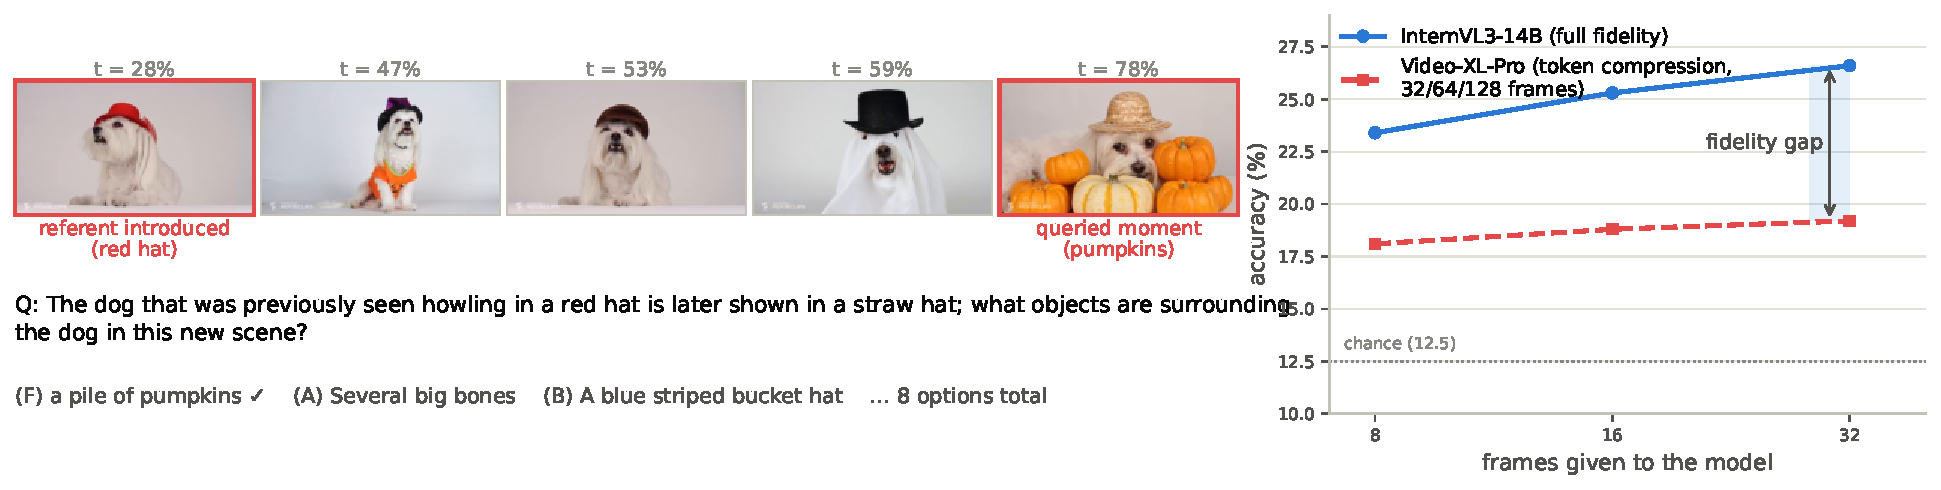
\includegraphics[width=\linewidth]{figures/fig1_teaser.pdf}
\caption{The \bench{} task and the headline finding. Left, a real benchmark item names a referent at one moment and asks about that referent after a scene cut, which forces re-identification followed by fine-grained reading. Right, a full-fidelity model (InternVL3-14B) improves with frame count while a token-compression model (Video-XL-Pro) stays near 19\%, a fidelity gap above 7 points.}
\label{fig:teaser}
\end{figure}

We evaluate \nummodels{} models. These span fifteen open-weight full-fidelity VLMs across six families \citep{internvl3,qwen25vl,gemma3,ovis,videollava,videochatflash}, four proprietary API models, and six long video models that compress visual tokens, four by learned summarization \citep{longvu,malmm,videoxl,videoxlpro} and two by state-space selective scan. The strongest model reaches 29.5\%, roughly double chance and far from solved. No question is answered by all \nummodels{} models, and 23.2\% are answered by none.

Our contribution is a diagnosis, not only a leaderboard. A benchmark named after re-identification invites the reading that models fail by confusing identities. We test that reading and reject it. Per-video accuracy is uncorrelated with the number of people on screen and with identity-switch opportunity, and twenty pipelines that ground the referent with dedicated re-identification models never beat the raw video. The bottleneck is coverage, not raw fidelity. More frames help every full-fidelity model, the older token-compression models stay flat near 19\% across a sixteen-fold frame increase, and lowering per-frame resolution to 112 pixels barely moves accuracy. That flatness is a property of the compression policy rather than of long video modeling as such, since two state-space models that compress selectively lead the open field. The ten-way taxonomy then localizes the failure, with role swaps at 13.9\% and multi-hop tracking at 16.1\% against easiest types near 20.6\%. Scale does not close the gap, since the parameter-to-accuracy correlation is 0.05. We release the benchmark, every model prediction, the shortcut audits, and the analysis code. Section~\ref{sec:method} sketches a re-identification-aware method that follows directly from the diagnosis and keeps the benchmark as the core contribution.

\section{Related Work}
\textbf{Long video models and token reduction.} Video LLMs began by aligning a vision encoder to a language model on short clips \citep{videollava,videochat,videochatgpt,llavaonevision,qwen2vl,qwen25vl,internvl25,internvl3,minicpmv,mplugowl3}. Scaling to long video forces a token budget that recent systems meet in different ways. MovieChat carries a dense-to-sparse memory across frames \citep{moviechat}; MA-LMM augments the model with a long-term memory bank \citep{malmm}; LongVU compresses spatiotemporally with adaptive frame selection \citep{longvu}; Video-XL and Video-XL-Pro reduce tokens by summarization and reconstructive compression \citep{videoxl,videoxlpro}; VideoChat-Flash applies hierarchical compression \citep{videochatflash}; LLaMA-VID uses two tokens per frame \citep{llamavid}; and Koala conditions on key frames \citep{koala}. HierarQ modulates features with a task-aware hierarchical querying transformer at a fixed token rate per frame \citep{hierarq}, and query-agnostic pruning methods allocate tokens by content \citep{apt,tome,fastv,prumerge}. A newer line replaces learned summarization with state-space sequence models, whose selective scan keeps a running summary at linear cost in sequence length. BIMBA compresses the visual token stream with a Mamba selective scan before the language model, and TimeViper interleaves Mamba and attention blocks so that long-range temporal state is carried by the recurrence while local detail stays attentive. We evaluate both, and they behave unlike the earlier compression models: they lead the open field on \bench{} rather than trailing it, which separates the question of how many tokens a long video model keeps from the question of which ones. We show why uniform compression fails on identity-grounded reading, and Section~\ref{sec:method} builds on query-conditioned selection \citep{flexselect,apt}.

\textbf{Long video benchmarks.} Existing suites evaluate global comprehension through plot, ordering, and coarse event questions \citep{videomme,mlvu,lvbench,longvideobench,egoschema,mvbench,activitynetqa,perceptiontest}. Reported accuracies of strong systems now exceed 80\% on several of them. A model family that reports 87.5\% on original MovieChat-1k questions scores below 20\% on \bench{} built from the same source videos. Needle-in-a-haystack protocols test retrieval of a planted item, which measures coverage rather than fine-grained identity reading. \bench{} differs by conditioning every question on tracking one referent across time.

\textbf{Language priors in multiple choice.} Multiple-choice video QA is vulnerable to text-only shortcuts, and language-only models often score far above chance \citep{goyal2017vqa,vqacp,annotationartifacts,atp,mmstar}. Single-frame baselines further solve many video questions without temporal reasoning \citep{atp}. We remove these shortcuts through committee filtering and report the full text-only and single-frame batteries with the benchmark.

\textbf{Person re-identification.} Re-identification is a mature retrieval field surveyed by \citet{reidsurvey}. TransReID introduces a pure transformer re-identification backbone \citep{transreid}; SOLIDER learns human-centric representations with semantic supervision \citep{solider}; CLIP-ReID adapts vision-language pretraining to re-identification \citep{clipreid}; OSNet learns omni-scale identity features \citep{osnet}; and Market-1501 and MEVID supply the image and video galleries these models use \citep{market1501,mevid}. Recent work targets hard shifts. DIFFER disentangles identity from clothing via semantic cues \citep{differ}; DisenQ disentangles biometric and non-biometric cues with a Q-Former \citep{disenq}; cloth-changing benchmarks LTCC, PRCC, and VC-Clothes stress appearance invariance \citep{ltcc,prcc,vcclothes}; and video benchmarks and methods such as MARS, TF-CLIP, and KeyRe-ID target temporal aggregation \citep{mars,tfclip,keyreid}. Temporal association is handled by multi-object trackers \citep{sort,bytetrack,botsort,deepocsort,strongsort}. We ask a different question, namely whether end-to-end VLMs possess this skill inside natural long video QA, and whether attaching dedicated re-identification pipelines helps. It does not, as Section~\ref{sec:notidentity} shows.

\section{The \bench{} Benchmark}
\label{sec:bench}

\textbf{Source and referents.} \bench{} is built over long videos drawn from three long-form collections, namely CinePile, the MovieChat-1k test split, and LVU, with a median length of 3.2 minutes and a median of 53 shot cuts per video. Movie footage cuts rapidly, so cross-shot identity persistence is native to the domain rather than an added perturbation. Referents are people in about three quarters of questions and animals in the rest. Thirty source videos could not be decoded by the local evaluation stack, so they and their 296 questions are excluded from every model and from all reported counts, which leaves the \numq{} questions over \numv{} videos evaluated here. Applying that exclusion to every model matters, because scoring undecodable items as wrong for local models while skipping them for API models understates open models by 1.1 to 2.2 points.

\textbf{Questions and tags.} Each question has eight options and one correct answer, with correct letters balanced across positions. We tag every question along four axes, summarized in Table~\ref{tab:composition}. The capability axis covers appearance, activity, location, interaction, and object state. The difficulty axis has 702 easy, 1362 medium, and 1603 hard questions, calibrated against measured accuracy in Appendix~\ref{app:diffcal}. The referral axis records how the referent is named. The challenge axis is a ten-way taxonomy of the re-identification skill required, which separates single-shot reference, cross-scene re-identification, long-term tracking, multi-hop tracking, appearance change, action sequences, spatial relationships, disambiguation among similar identities, occlusion recovery, and role or position swaps.

\textbf{Protocol.} Models receive the question, the eight options, and frames sampled uniformly from the full video. The standard budget is eight frames, and we ablate 16, 32, 64, and 128. Models output one option letter, parsed by a shared routine and scored by exact match, and a model's own unparseable output counts as wrong. Every model runs zero-shot, and no model is trained on \bench{} videos or questions.

\begin{table}[t]
\centering
\caption{Composition of \bench{} along its capability and re-identification challenge axes. The full distributions of all four axes appear in Appendix~\ref{app:composition}.}
\label{tab:composition}
\small
\begin{tabular}{@{}lr@{\hspace{22pt}}lr@{}}
\toprule
\rowcolor{sectiongray}
\multicolumn{2}{c}{\textbf{Capability}} & \multicolumn{2}{c}{\textbf{Re-identification challenge}} \\
\midrule
Location & 849 & Cross-scene re-identification & 1092 \\
Activity & 750 & Single-shot reference & 515 \\
Appearance & 721 & Multi-hop tracking & 504 \\
Interaction & 696 & Appearance change & 442 \\
Object state & 651 & Long-term tracking & 384 \\
 & & Action sequence & 328 \\
 & & Spatial relationship & 265 \\
 & & Disambiguation, similar & 100 \\
 & & Occlusion recovery & 26 \\
 & & Role or position swap & 11 \\
\bottomrule
\end{tabular}
\end{table}

\section{Main Results and Analysis}
\label{sec:results_analysis}
Table~\ref{tab:leaderboard} reports the leaderboard. Three facts frame the analysis.

\textbf{The benchmark is hard and unsaturated.} The strongest model is the proprietary GPT-5.5 at 29.5\%, and the best open model is TimeViper at 27.2\%, a hybrid Mamba-Transformer long video model rather than a full-fidelity VLM. Several widely used models sit within a few points of the \chance{} chance level. On the common subset answered by all \nummodels{} models, no question is solved by every model and 23.2\% are solved by none. GPT-5.5's content filter declined 528 questions and it answers repeated items inconsistently, so its score is computed over the 3{,}139 distinct questions it attempted, with its unparseable responses counted wrong; all skip protocols appear in Section~\ref{sec:quality}.

\textbf{Scale does not buy the skill.} The Pearson correlation between log parameters and accuracy is 0.05 across all models and 0.16 within full-fidelity open models, shown in right panel of Figure~\ref{fig:results2} and by family in Appendix~\ref{app:scalefamily}. Scaling inside a family adds little, since InternVL3 gains 4.5 points from 2B to 14B, and family dominates, since InternVL3-2B at 20.9\% beats three 8B models from other families.

\textbf{Compression architecture decides whether a long video model trails.} The long-video group splits in two. The four older token-compression models occupy the bottom of the board between 11.3\% and 19.2\% despite reading 128 frames against the default eight, but the two recent state-space designs sit at the top of the open field: TimeViper, a hybrid Mamba-Transformer, reaches 27.2\% and is the best open model overall, and BIMBA, which compresses tokens with a Mamba selective scan, reaches 25.1\%. Both beat every full-fidelity open VLM while reading far more frames, so long video architecture is not intrinsically disqualifying for identity-grounded reading. What separates them is what the compression preserves rather than how much it discards, which is the distinction Section~\ref{sec:p3} measures directly: the models whose memories are evidence-blind lose the answer, and the selective-scan designs that keep a query-relevant summary do not. The left panel of Figure~\ref{fig:results2} shows the per-capability picture, where all groups still collapse together on the tracking-heavy axes, so no architecture escapes the benchmark's core difficulty. Section~\ref{sec:coverage} attributes the older models' deficit to a fidelity cost of compression rather than a data or scale artifact.

\begin{figure}[t]
\centering
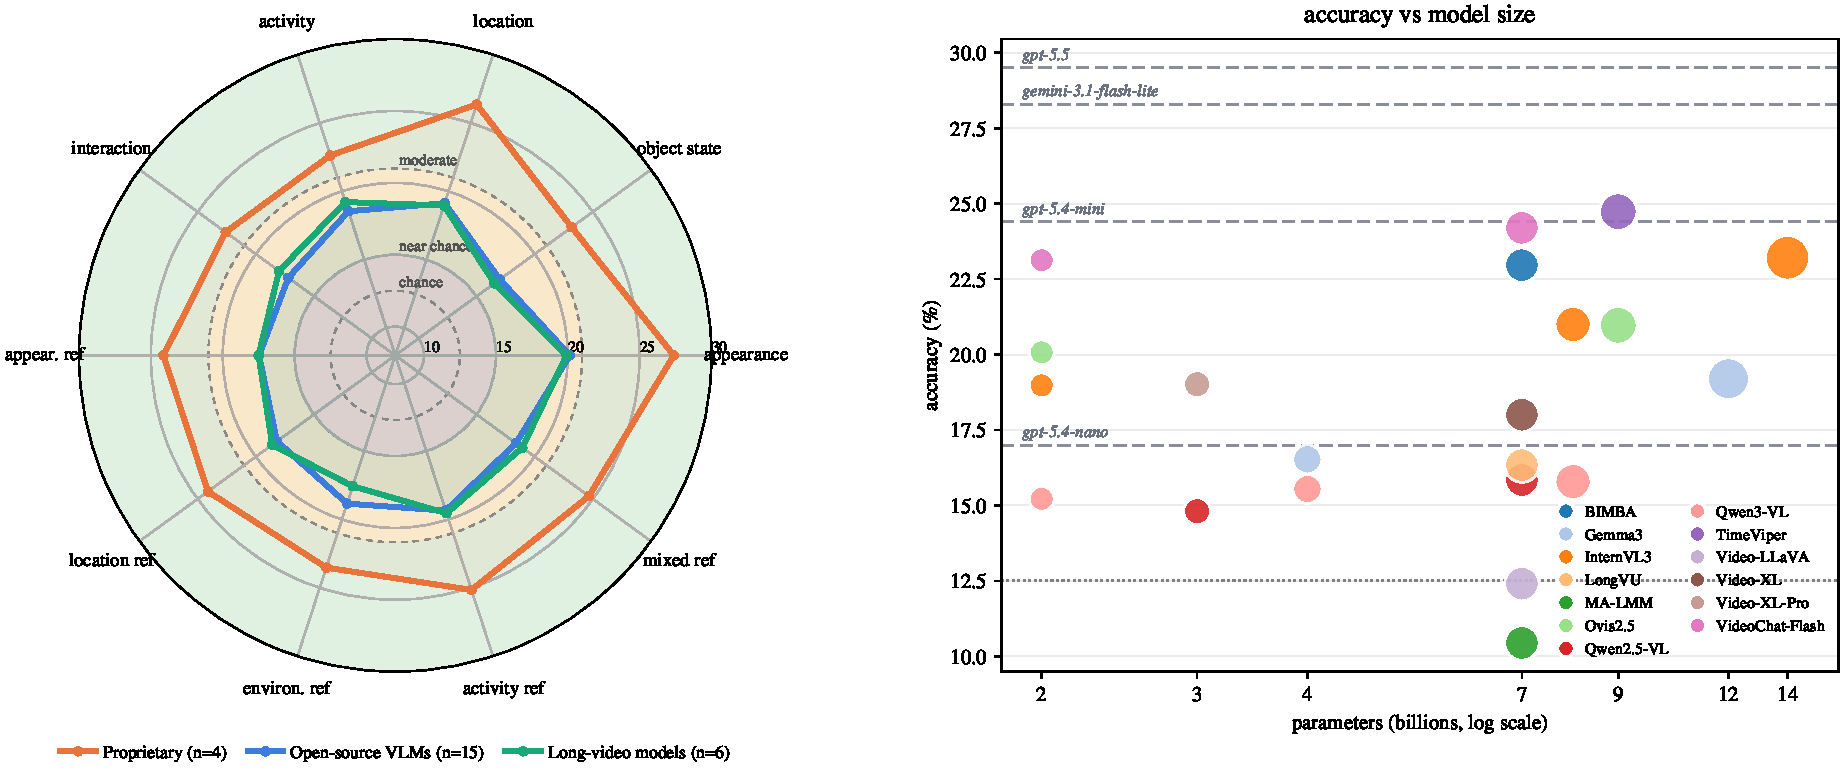
\includegraphics[width=\linewidth]{figures/fig_radar_bubble.pdf}
\caption{Left, accuracy on each capability and referral axis, averaged within the three model groups of Table~\ref{tab:leaderboard}, namely four proprietary models, fifteen open-source VLMs, and four long-video token-compression models, against the \chance{} chance level with shaded difficulty bands. Proprietary models reach the moderate band on every axis, open-source VLMs sit inside them, and long-video models sit inside both near chance, and all three groups are weakest on the same tracking-heavy axes. Right, accuracy against parameter count, where scale is a weak predictor at $r=0.05$ and family dominates.}
\label{fig:results2}
\end{figure}

\begin{table}[t]
\centering
\caption{\bench{} leaderboard at each model's evaluation frame budget. Accuracy is against a \chance{} chance level, best per group in bold. All models are scored on the same \numq{} questions, since the thirty undecodable videos are excluded everywhere. Per-model N still varies for the API models, whose content filters decline items, and common-subset comparisons appear in Section~\ref{sec:results_analysis}. $^{\dagger}$GPT-5.5 declined 528 questions and answers repeats inconsistently; its score is over the 3{,}139 distinct questions it attempted, counting unparseable responses wrong.}
\label{tab:leaderboard}
\small
\begin{tabular}{@{}lccc@{}}
\toprule
Model & Size & Frames & Acc (\%) \\
\midrule
\rowcolor{sectiongray}
\multicolumn{4}{c}{\textbf{Proprietary models}} \\
\midrule
\rowcolor{highlightgreen}
GPT-5.5$^{\dagger}$ & -- & 8 & \textbf{29.5} \\
Gemini-3.1-Flash-Lite & -- & 8 & 28.2 \\
GPT-5.4-mini & -- & 8 & 24.4 \\
GPT-5.4-nano & -- & 8 & 17.0 \\
\midrule
\rowcolor{sectiongray}
\multicolumn{4}{c}{\textbf{Open-source VLMs }} \\
\midrule
\rowcolor{highlightgreen}
VideoChat-Flash-7B & 7B & 8 & \textbf{26.4} \\
InternVL3-14B & 14B & 8 & 25.4 \\
VideoChat-Flash-2B & 2B & 8 & 25.4 \\
InternVL3-8B & 8B & 8 & 23.1 \\
Ovis2.5-9B & 9B & 8 & 23.0 \\
Ovis2.5-2B & 2B & 8 & 22.2 \\
Gemma3-12B & 12B & 8 & 21.3 \\
InternVL3-2B & 2B & 8 & 20.9 \\
Gemma3-4B & 4B & 8 & 18.2 \\
Qwen2.5-VL-7B & 7B & 8 & 17.5 \\
Qwen3-VL-8B & 8B & 8 & 17.4 \\
Qwen3-VL-4B & 4B & 8 & 17.0 \\
Qwen3-VL-2B & 2B & 8 & 16.6 \\
Qwen2.5-VL-3B & 3B & 8 & 16.2 \\
Video-LLaVA & 7B & 8 & 13.6 \\
\midrule
\rowcolor{sectiongray}
\multicolumn{4}{c}{\textbf{Long-video models (incl. state-space compression)}} \\
\midrule
\rowcolor{highlightgreen}
TimeViper (hybrid Mamba-Transformer) & 9B & 1 FPS & \textbf{27.2} \\
BIMBA (Mamba selective-scan) & 7B & 64 & 25.1 \\
Video-XL-Pro & 3B & 128 & 19.2 \\
Video-XL & 7B & 128 & 18.1 \\
LongVU (Qwen2) & 7B & 1 FPS & 17.9 \\
MA-LMM & 7B & 20 & 11.3 \\
\midrule
\emph{Chance} & & & 12.5 \\
\bottomrule
\end{tabular}
\end{table}


Each subsection states a question, runs a test, reports the number, and draws one implication. Correlations are Pearson. We read correlation $r$ below 0.3 as weak, 0.3 to 0.7 as moderate, and above 0.7 as strong. Binned curves drop bins with fewer than 20 items, and intervals are bootstrap percentile intervals over questions.

\subsection{Which re-identification skills do models lack?}
\label{sec:skills}
The benchmark is named for re-identification and sits far below ceiling, so the first question is which re-identification skills break. The challenge taxonomy exposes a stable skill hierarchy across all \nummodels{} models (full per-model heatmap in Appendix, see Figure~\ref{fig:reidslice}). Role and position swaps score 13.9\% against a \chance{} chance level, and multi-hop tracking scores 16.1\%. Long-term tracking and disambiguation among similar identities follow at 18.1\%. Single-scene and appearance types are easiest near 20.6\%. Models can recognize a described person, since single-shot and appearance questions are the most answerable. Models cannot maintain identity through temporal structure, since chains of references, swaps, and long gaps are hardest. These are the cases where the answer depends on frames that uniform sampling tends to miss. Figure~\ref{fig:gallery} shows three failures, all missed by InternVL3-14B and Gemini-3.1-Flash-Lite.

\begin{figure}[t]
\centering
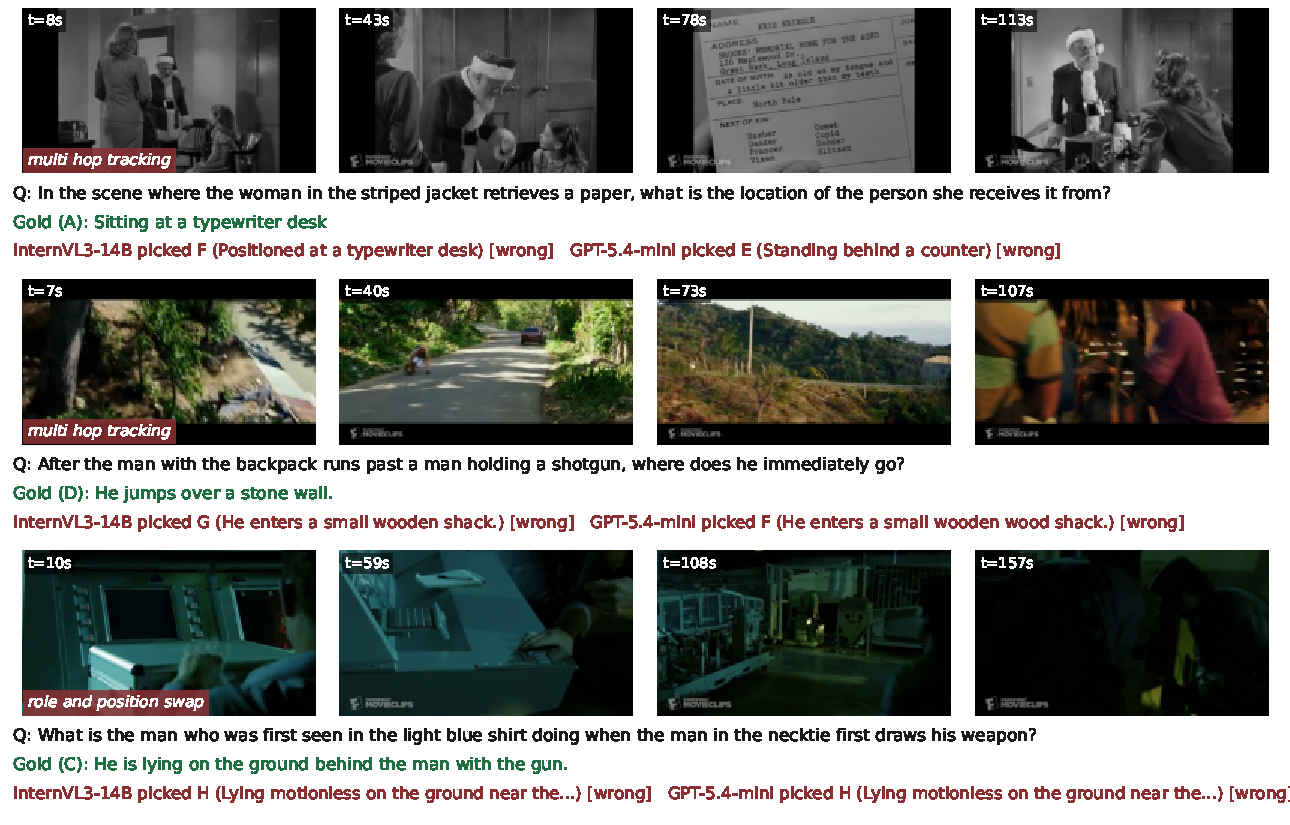
\includegraphics[width=\linewidth]{figures/fig_gallery.pdf}
\caption{Three failures on tracking-heavy questions. Frames appear left to right, with the question, ground-truth answer, and the letters chosen by InternVL3-14B and GPT-5.4-mini below each row.}
\label{fig:gallery}
\end{figure}

\subsection{Difficulty is not identity confusion}
\label{sec:notidentity}
The hardest skills in Section~\ref{sec:skills} all involve tracking, which points to identity confusion as the cause. We test that hypothesis three ways and reject each. More people on screen do not make questions harder. Per-video accuracy averaged over models correlates at $r=0.02$ with concurrent-person count and at $r=0.02$ with an identity-switch-opportunity score, shown across every measured video property in Appendix~\ref{app:drivers} (Figure~\ref{fig:driversmulti}). The only moderate correlates are duration and visual variability, both at $r=0.42$ and positive, so longer and more varied videos are slightly easier. Difficulty on \bench{} is not explained by opportunities for identity confusion. Question wording, referral, and referent type do not concentrate difficulty either (Appendix~\ref{app:qhardness}), nor is it tied to any visual-content cluster (Appendix~\ref{app:landscape}).

Doing the identity bookkeeping for the model does not help either. We build a three-stage pipeline that detects and tracks every person and animal with four trackers, links tracklets across shots into global identities with generic CLIP features or one of four dedicated re-identification models, grounds the referent to one identity, and renders a clip that marks only that identity. Each of the twenty pipelines runs with all seventeen local models, reported in Appendix~\ref{app:reid} (Table~\ref{tab:reid}). Every pipeline sits at or below the 19.7\% raw-video baseline. Tracker choice moves accuracy by at most 0.6 points, and dedicated re-identification models are slightly worse than generic CLIP linking. The strongest VLMs lose up to 6 points, because cropping to one identity discards scene context they exploit. Identity-tracking quality is not the limiting factor.

Errors are systematic. When models err, 52\% of wrong answers land on a single modal distractor, against 14\% expected under uniform error, and the pairwise correlation between model correctness vectors averages $\phi=0.24$ with a maximum of 0.54, shown in Appendix~\ref{app:diffcal} (Figure~\ref{fig:agree}). Models share a failure mode rather than making independent identity mix-ups.

\subsection{Mechanistic probes}
\label{app:attention}
Four probes on InternVL3-8B, a representative open full-fidelity model, explain why coverage governs accuracy and raw resolution does not. We instrument the model with attention hooks and read the attention from the generated answer tokens back to the visual tokens of each frame, averaged over heads. Figure~\ref{fig:attn}a shows that this attention concentrates on the last frames and places only 3 to 5\% of its total mass on visual tokens, so the model both misses relevant moments through sparse sampling and underweights the frames it does receive. The recency bias holds at 8 and 32 frames and persists even when the final frame is a closing card rather than content, which is why simply adding frames does not repair accuracy. This matters for the coverage story because it shows that unread frames, not unavailable frames, cap accuracy.
\begin{figure}[h]
\centering
\begin{subfigure}{0.78\linewidth}\centering
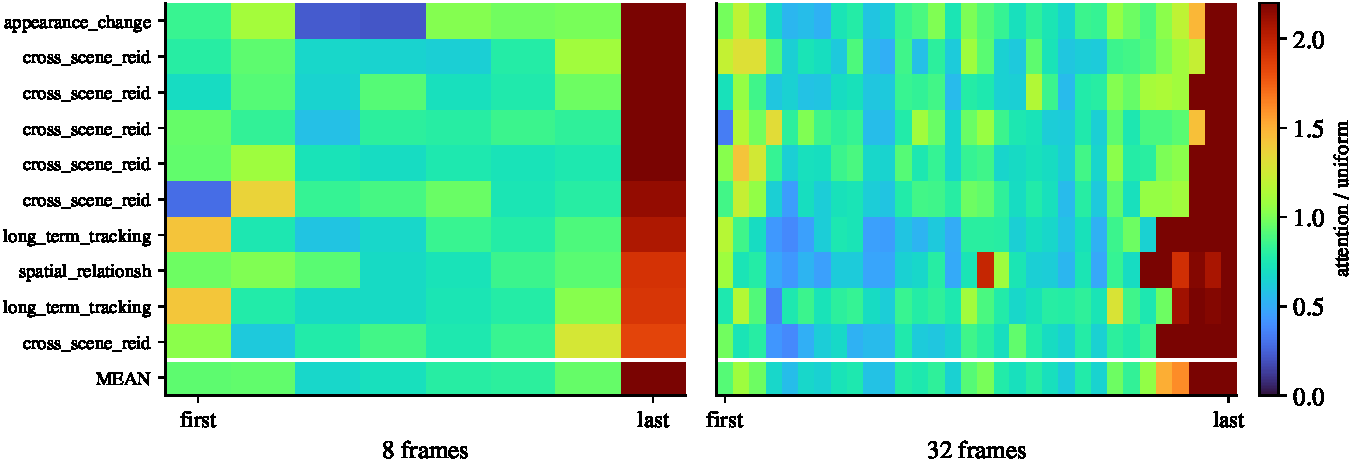
\includegraphics[width=\linewidth]{figures/fig_attention_frames.pdf}
\caption{Attention over frame position}\label{fig:attnframes}
\end{subfigure}\\[3pt]
\begin{subfigure}{0.92\linewidth}\centering
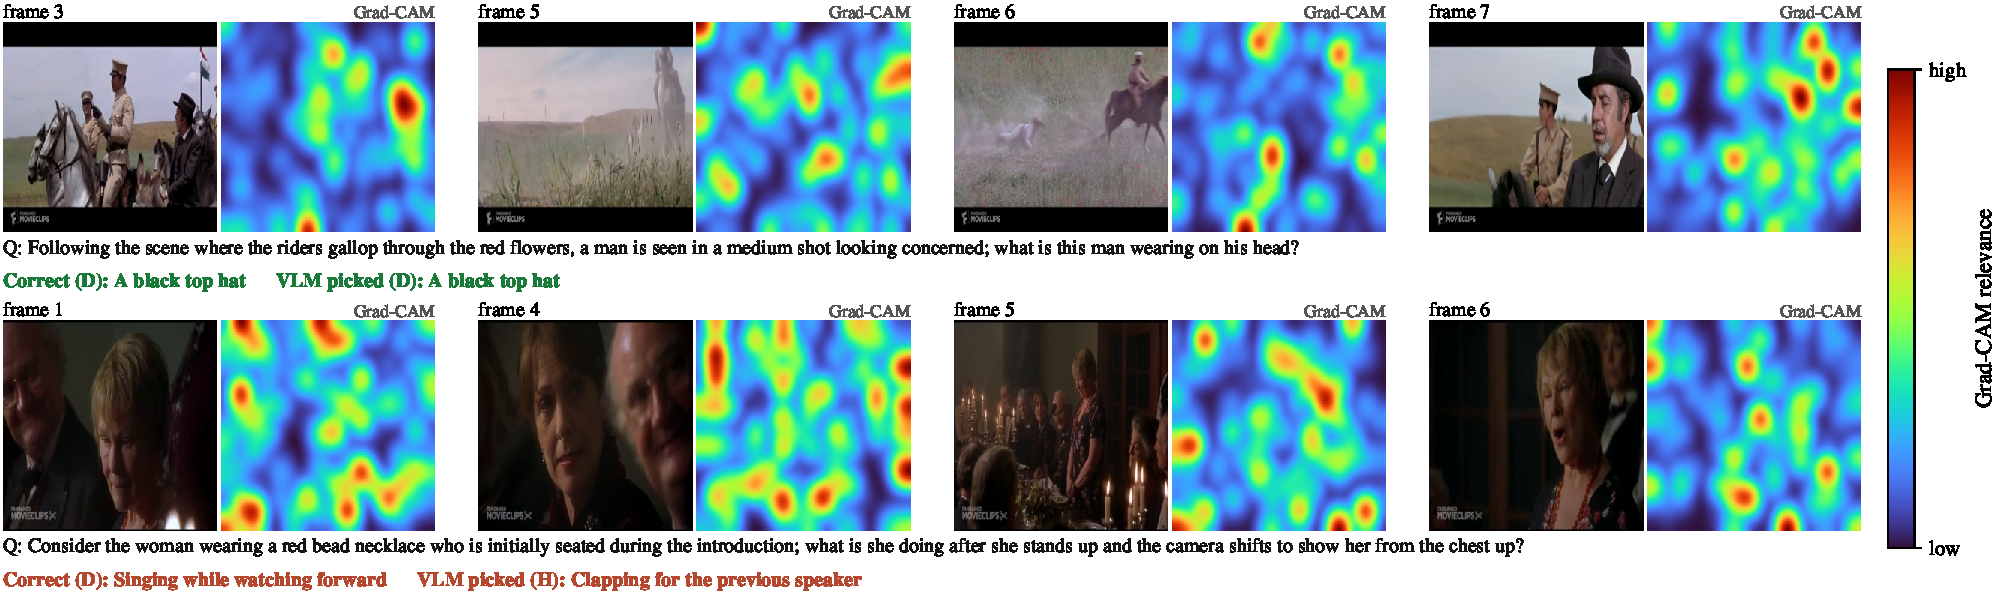
\includegraphics[width=\linewidth]{figures/fig_gradcam_regions.pdf}
\caption{Grad-CAM for spatial relevancy}\label{fig:gradcam}
\end{subfigure}
\caption{(a) Per-question attention from answer tokens to each frame at 8 and 32 frames, sorted by last-frame mass with the mean row at the bottom. Attention concentrates on the final frame regardless of content. (b) Spatial relevancy on the peakiest correct and wrong examples, per-frame normalized. Correct answers place hot spots on the referent, wrong answers scatter to background and outro cards.}
\label{fig:attn}
\end{figure}

We then map attention onto the native sixteen by sixteen vision patch grid to see where inside each frame the model looks. Figure~\ref{fig:attn} depicts the attention maps to show relevancy on the peakiest correct and wrong examples. Correct answers place hot spots on the referent, while wrong answers scatter across background and outro cards, which is the spatial counterpart of the frame-level recency bias. Figure~\ref{fig:tsne} embeds a 64-frame pool per video with a CLIP encoder and marks the clusters an 8-frame and a 32-frame uniform sample reach, which visualizes the coverage gap. Figure~\ref{fig:layerwise} then follows the same failure inward through the language model. Panel (a) tracks the cosine similarity between visual-token representations at reduced budgets and the 32-frame reference across layers, and the dip in middle layers shows where missing coverage enters the representation. Panel (c) reads the answer-token attention on the referent frame at increasing depth, where it starts diffuse, sharpens onto the referent by the middle layers, and then stays on the person for correct answers but drifts to the background for wrong ones. Panel (b) applies a logit lens to the answer position and shows the correct option gains probability only in the last few layers when the model succeeds, while in failures it never rises and the chosen wrong option does, so the decision is committed late and downstream of evidence that is already lost. Together the probes trace one causal chain, namely sparse sampling misses scene clusters, recency-biased attention underreads the frames that arrive, spatial relevancy lands off the referent and drifts further off it with depth, the representation gap opens in the middle layers, and the answer is fixed in the last layers with the correct option no longer recoverable. All of this runs on one representative model, so it explains a mechanism rather than establishes a population law, and the chain is read as an existence proof that unread frames, not unavailable frames, cap accuracy. Attention mass is read from generated answer tokens back to visual tokens and averaged over heads, which understates any single sharp head but is robust to head-level noise.

\begin{figure}[h]
\centering
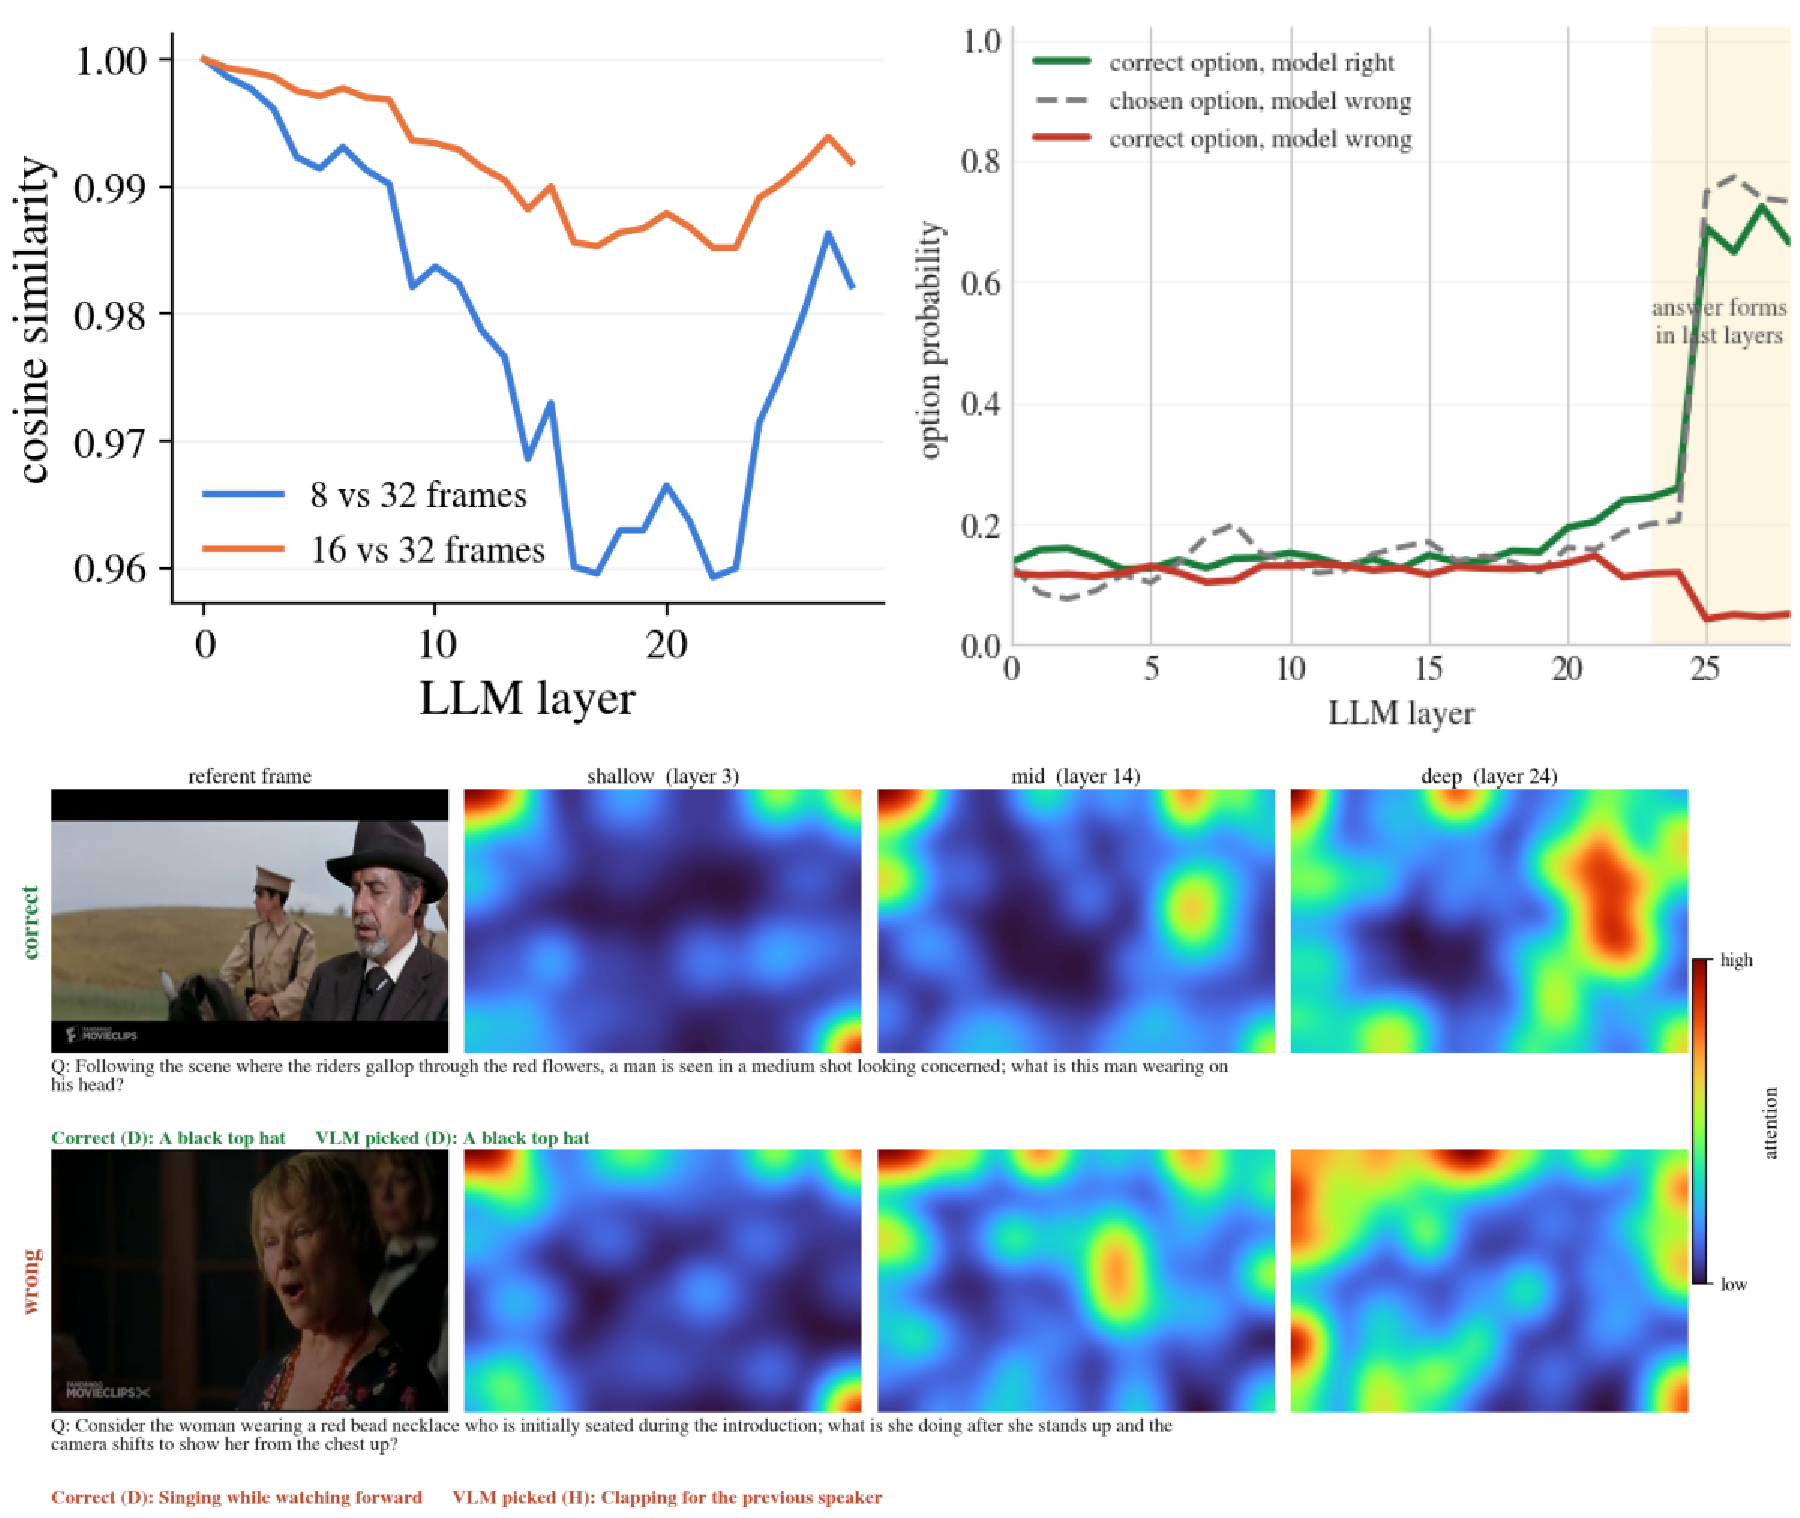
\includegraphics[width=0.8\linewidth]{figures/fig_mechanism_depth.pdf}
\caption{Following the failure inward on InternVL3-8B. (a) Cosine similarity of visual-token representations at reduced frame budgets against the 32-frame reference, layer by layer, where the middle-layer dip marks where missing coverage enters the representation. (b) Logit-lens readout of the option probabilities at each layer, averaged over questions the model answers right and wrong, where the correct option becomes probable only in the last few layers when the model succeeds and in failures never rises while the chosen wrong option does. (c) Answer-token spatial attention on the referent frame at a shallow, a middle, and a deep layer, sharpening onto the referent for the correct answer and drifting to the background for the wrong one.}
\label{fig:layerwise}
\end{figure}
\subsection{The bottleneck is coverage, not raw fidelity}
\label{sec:coverage}
If identity confusion is not the cause, the alternative is that models never see or never resolve the right pixels. This subsection isolates the two halves of that alternative, temporal coverage and per-frame fidelity. Coverage helps monotonically. Raising uniform frames from 8 to 16 to 32 lifts every full-fidelity model tested, and InternVL3-14B goes 25.4, 27.3, 28.6, shown in Figure~\ref{fig:coverage} and across seven models in Appendix~\ref{app:covmulti}. Compression buys coverage by destroying the fidelity this task needs. Video-XL-Pro reads 32 to 512 frames through reconstructive compression, yet its accuracy stays between 18.1\% and 19.2\% across the sweep, so a sixteen-fold frame increase adds nothing. Thirty-two full-fidelity frames beat 512 compressed frames by more than 7 points.

Raw per-frame resolution is a weak lever. Holding the budget at 32 frames and lowering resolution keeps accuracy flat from 448 to 112 pixels, and it drops up to 2.8 points only at 56 pixels for the larger models, while InternVL3-2B stays flat from 15.8\% to 15.6\%, shown in Figure~\ref{fig:fidelity}. Compression models therefore do not fail from low pixel resolution. They fail by spending the token budget on the wrong content, which the coverage and selection results establish. Two mechanisms explain the coverage loss. Uniform sampling covers only 57.3\% of a video's scene clusters at 8 frames, 75.3\% at 16, and 89.2\% at 32, shown in Figure~\ref{fig:collapse} and confirmed by the t-SNE clusters in Figure~\ref{fig:tsne}.

Selecting the right frames beats sampling more of them. A training-free probe scores 64 candidate frames against the question with CLIP and keeps the top eight, which adds 1.0 to 2.7 points on three families at a fixed eight-frame budget. Selection compounds with coverage, since selected 16 and 32 frames beat uniform 16 and 32, and the best configuration reaches 31.4\%, shown in Figure~\ref{fig:coverage}. The same external selection hurts the one model with native internal frame handling, since VideoChat-Flash drops 3.0 points, so selection must live inside the model. An oracle over five frame strategies reaches about 40\%, which bounds how much of the remaining error is a frame-choice problem.

\begin{figure}[t]
\centering
\begin{subfigure}{0.33\linewidth}\centering
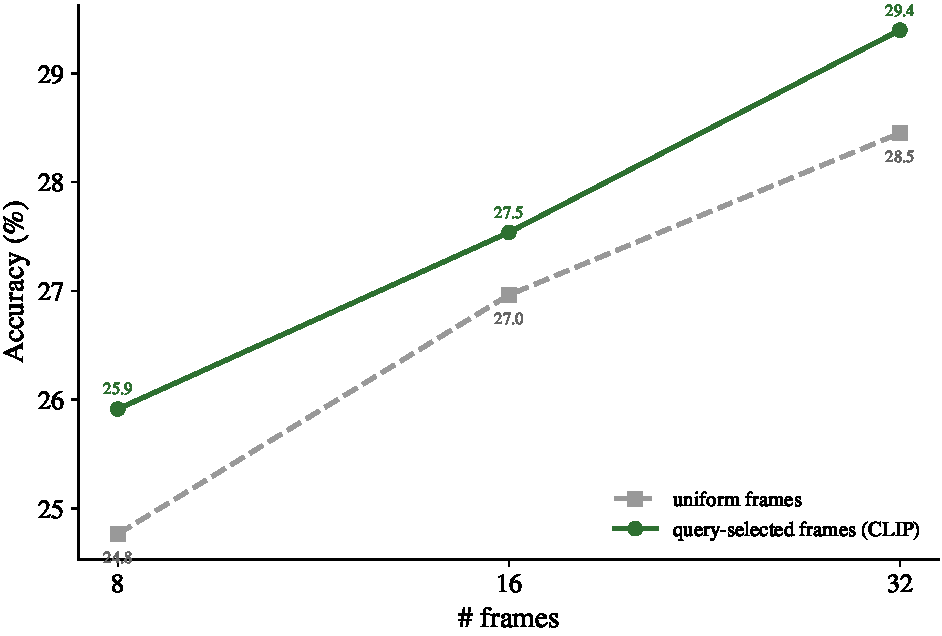
\includegraphics[width=\linewidth]{figures/fig_selection_vs_coverage.pdf}
\caption{Coverage and selection}\label{fig:coverage}
\end{subfigure}\hfill
\begin{subfigure}{0.33\linewidth}\centering
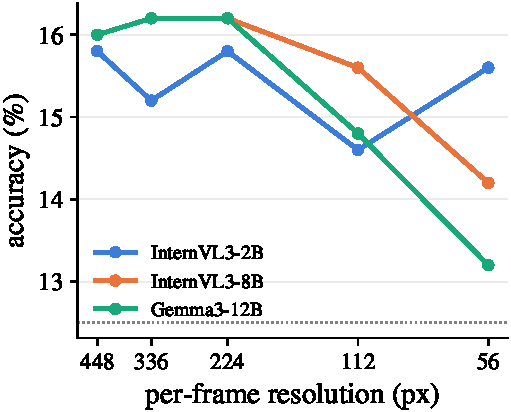
\includegraphics[width=\linewidth]{figures/fig_resolution_sweep.pdf}
\caption{Fidelity sweep}\label{fig:fidelity}
\end{subfigure}\hfill
\begin{subfigure}{0.33\linewidth}\centering
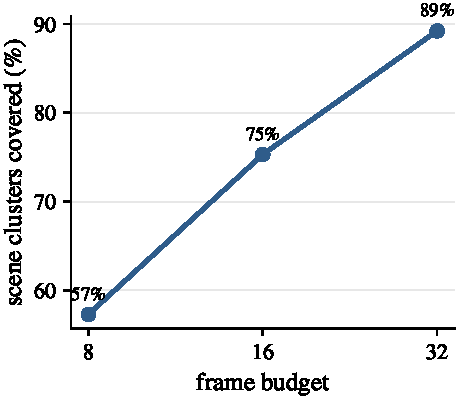
\includegraphics[width=\linewidth]{figures/fig_feature_collapse.pdf}
\caption{Scene coverage}\label{fig:collapse}
\end{subfigure}
\caption{Coverage decides performance, raw resolution does not. Left, query-selected frames beat uniform frames at every budget on InternVL3-14B. Middle, accuracy is flat as per-frame resolution drops from 448 to 112 pixels at a fixed 32-frame budget. Right, uniform sampling covers a shrinking fraction of a video's scene clusters as the budget falls.}
\label{fig:coverfid}
\end{figure}

\subsection{Necessity and robustness}
\label{sec:necessity}
The controlled probes below run on four models that expose frame-level control, namely InternVL3-2B, InternVL3-8B, InternVL3-14B, and Gemma3-12B. Qwen2.5-VL-7B and VideoChat-Flash-7B are excluded because they handle frame sampling internally and returned no valid predictions under frame manipulation.

Coverage matters only if the questions genuinely need temporal evidence, so we test necessity first and robustness second. The task requires temporal evidence. Moving from 1 to 8 frames lifts InternVL3-2B from 11.0\% to 17.2\%, a gain of 6.2 points, and InternVL3-8B from 11.8\% to 16.0\%, a gain of 4.2 points, shown across challenge types in Figure~\ref{fig:tneed}. A single frame scores near the \chance{} chance level, so \bench{} answers the single-frame-bias critique of video QA \citep{atp}. Coverage helps unevenly across challenge types, so added frames pay off most where the answer is spread across time and least where a single reference frame already carries it, quantified per challenge type in Appendix~\ref{app:perchalcov}.

Models use temporal order, but weakly. Shuffling the eight frames lowers InternVL3-2B by 1.8 points and reversing them lowers it by 2.8 points, shown in Figure~\ref{fig:torder}. The effect shrinks with model size and reaches about zero for InternVL3-14B. Order therefore carries a weak signal that larger models rely on less, which matches the tracking failures in Section~\ref{sec:skills}.

Answers are fragile to input degradation and option order. Blur, JPEG, and Gaussian noise lower accuracy by up to 4.5 points, moving InternVL3-2B from 17.8\% clean to 13.2\% under noise, while downscaling to 112 pixels is nearly lossless, shown per model in Figure~\ref{fig:robust}. Rotating the option contents by three positions leaves accuracy near flat, yet the model changes its content answer on 49.8\% of questions, shown in Figure~\ref{fig:optsens}, so the choice is unstable even when accuracy looks stable.

\begin{figure}[h]
\centering
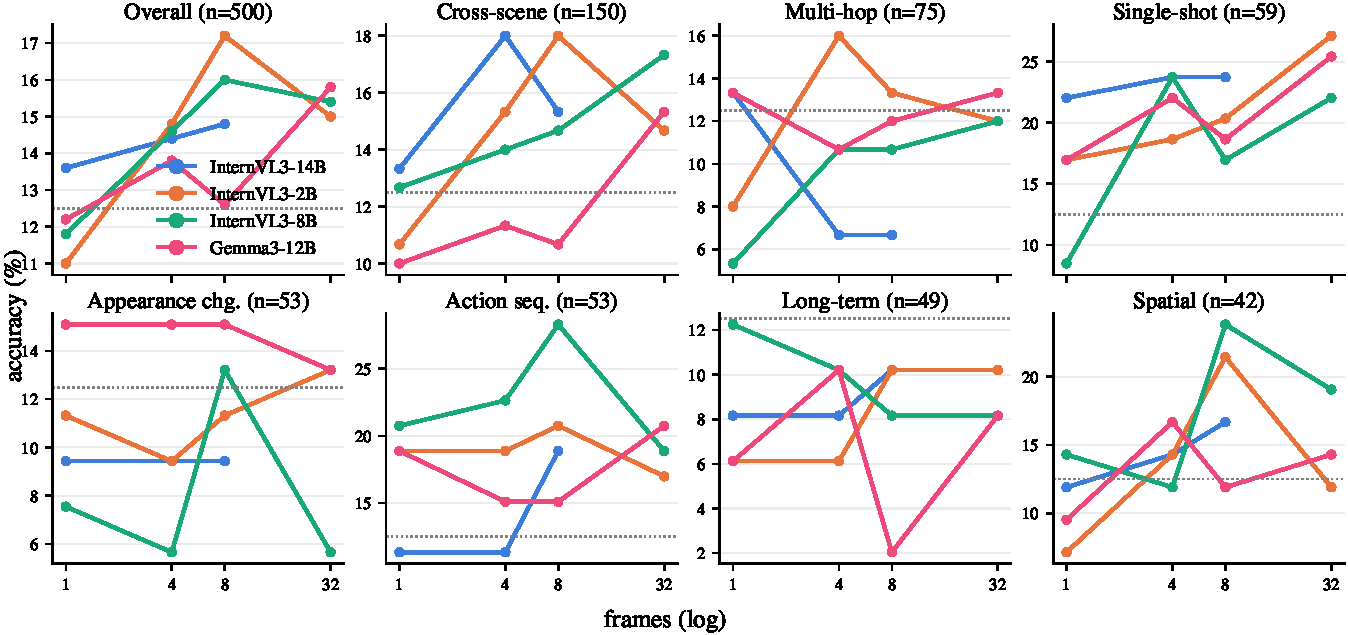
\includegraphics[width=\linewidth]{figures/fig_temporal_necessity.pdf}
\caption{Temporal necessity by challenge type, a small-multiples grid over the four frame-control models. Each panel plots accuracy against the frame budget for one challenge type with its question count. Every panel rises from 1 frame, so a single frame is insufficient, and the size of the gain varies by challenge type.}
\label{fig:tneed}
\end{figure}

These three probes appear in full in Figure~\ref{fig:robbattery}, with per-model breakdowns and interpretation in Appendix~\ref{app:corruption}.
\begin{figure}[t]
\centering
\begin{subfigure}[b]{0.27\linewidth}\centering
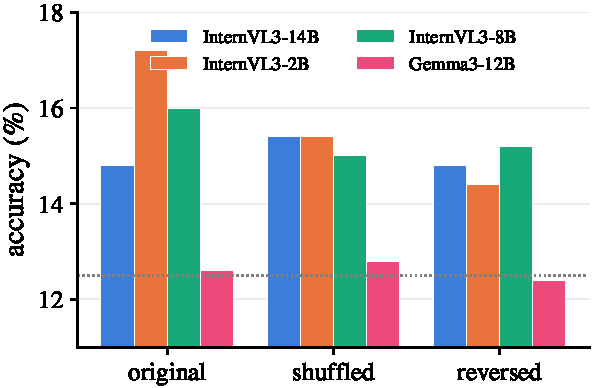
\includegraphics[width=\linewidth]{figures/fig_temporal_order.pdf}
\caption{Temporal order}\label{fig:torder}
\end{subfigure}\hfill
\begin{subfigure}[b]{0.27\linewidth}\centering
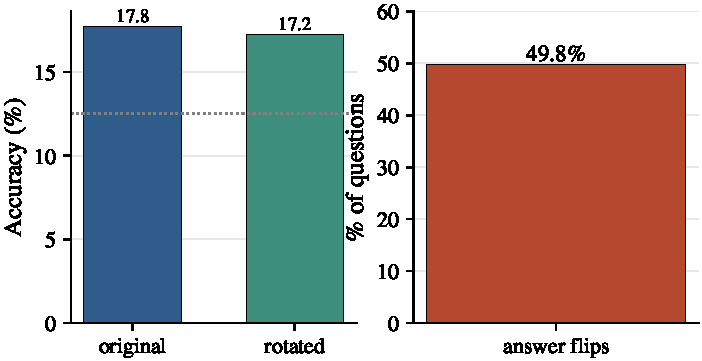
\includegraphics[width=\linewidth]{figures/fig_option_sensitivity.pdf}
\caption{Option order}\label{fig:optsens}
\end{subfigure}\hfill
\begin{subfigure}[b]{0.42\linewidth}\centering
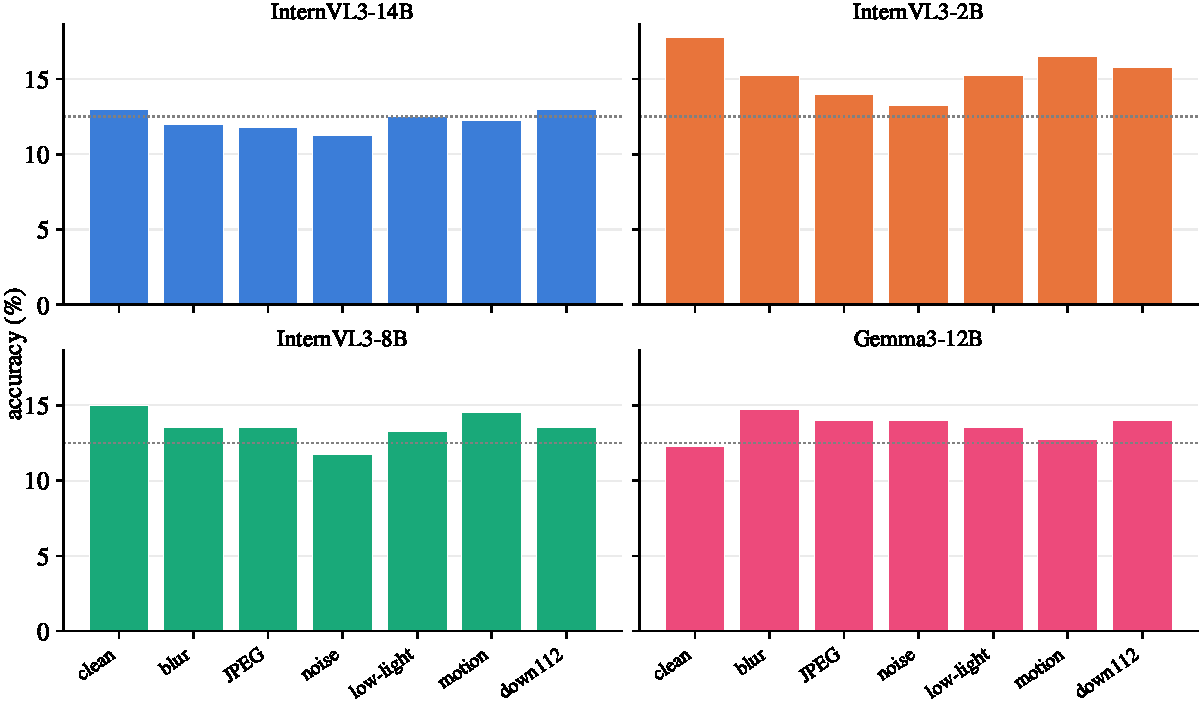
\includegraphics[width=\linewidth]{figures/fig_corruption.pdf}
\caption{Input corruption, one panel per model}\label{fig:robust}
\end{subfigure}
\caption{Robustness batteries on the four frame-control models. (a) Shuffling or reversing the eight frames lowers accuracy by 1.8 to 2.8 points on InternVL3-2B and by about zero on InternVL3-14B. (b) Rotating the option contents by three positions leaves accuracy near flat while changing the chosen content answer on 49.8\% of questions. (c) Six corruptions at a fixed reduced-resolution probe setting, so panels report relative drops, lower accuracy by up to 4.5 points while downscaling to 112 pixels is nearly lossless.}
\label{fig:robbattery}
\end{figure}

\subsection{Benchmark quality}
\label{sec:quality}
The findings above are only trustworthy if the benchmark itself is well-behaved, so we close with three checks on stability, significance, and cost. Rankings are stable across evaluation budgets. The Spearman correlation between leaderboards at 8, 16, and 32 frames is 0.95 to 0.99, so conclusions do not depend on the frame budget. Headline numbers carry bootstrap intervals, resampled over videos rather than questions because questions from one video are not independent. GPT-5.5 at 29.5\% has a 95\% interval of 27.5 to 31.4, above the interval of GPT-5.4-mini at 22.9 to 25.9, so its lead is significant. Role and position swaps have an interval of 4.1 to 25.2 that includes chance, which confirms that slice sits at chance. GPT-5.5's denominator deserves care, because its raw output repeats 65 question keys and answers 55 of them inconsistently on the second pass, so the model is not deterministic on this task. Scoring instead moves it to 30.7\% when its unparseable responses are excluded rather than counted wrong, 25.2\% when all 528 declined questions are scored wrong, and 27.5\% when declined questions are assigned chance; we report the first column as the headline and state all four, because a single column is misleading. Evaluating a proprietary model on the full benchmark costs between 0.5 and 7 US dollars, so \bench{} is practical for repeated use.

\section{Where the Failures Come From: Three Diagnostic Analyses}
\label{sec:diagnostics}
The results so far say what fails. This section asks why, with three diagnostics that each isolate one suspected cause. First, whether models can re-identify a person at all, split into what their features store and what their answers use. Second, whether uniform sampling ever shows the model the frames that carry the answer, turned from a proxy into a measured and causally tested quantity. Third, for the models that compress visual tokens into a memory, whether the evidence is destroyed by the compression or stored but never retrieved. The three answers combine into a single failure chain that explains both the leaderboard and the limits of input-side fixes.

\subsection{Models store identity but cannot answer with it}
\label{sec:p1}
\textbf{Setup.} We build a bank of 7{,}055 person crops from the tracker outputs of Appendix~\ref{app:reid} (114 videos) and form 2{,}848 balanced same-or-different-person pairs, where the two crops of a pair come from the same video at time gaps from ten seconds to over two minutes and different-person pairs are drawn from the same video so background cues do not give the answer away. Each pair is pasted side by side into one image, and every model answers \emph{is this the same individual, yes or no} through the exact multiple-choice path it uses on the benchmark. As a reference we score the same pairs by the cosine similarity of frozen CLIP ViT-B/32 image embeddings \citep{clip} with a cross-validated threshold, so the reference has no language model at all.

\textbf{Models barely beat a coin flip where a frozen encoder does not.} VLM accuracy spans 50.6\% (Gemma3-12B, exactly a coin flip) to 62.6\% (InternVL3-14B), while the 150M-parameter CLIP reference reaches 85.2\% on the identical pairs (Figure~\ref{fig:reidprobe}, left). VLM accuracy also decays as the time gap between the two crops grows, while the CLIP reference stays flat (Figure~\ref{fig:reidprobe}, right), so the failure worsens exactly in the long-gap regime the benchmark tests.

\textbf{The identity information is inside the model.} We embed every crop with the model's own vision features, taken at the point where they enter the language model, and measure within-video identity retrieval, meaning how often the most similar other crop shows the same person. We report CMC@1 and mAP, the standard re-identification retrieval metrics \citep{market1501,reidsurvey}, where CMC@1 is the rank-1 hit rate. InternVL3-8B's features reach 84.5 CMC@1 and 74.6 mAP, yet the same model answers the behavioral probe at 61.6\%. The information survives the vision encoder and is lost at answering, a read-out gap of about 23 points. Figure~\ref{fig:constellation} visualizes the feature space of one video, where identities form clean islands and the model's errors connect crops that share clothing rather than identity. The characteristic error is outfit matching. In the showcase of Figure~\ref{fig:reidprobe}, two different men wearing the same blue shirt are declared the same person, and even the feature similarity of that pair (0.89) matches the same-person median (0.90), so appearance overwhelms identity in exactly the case re-identification exists to solve \citep{osnet,ltcc}. This also explains Section~\ref{sec:notidentity}: external re-identification pipelines cannot help a model that fails to consume identity evidence at answer time, not because identity association is hard but because the model discards it.

\begin{figure}[t]
\centering
\begin{subfigure}[b]{0.60\linewidth}\centering
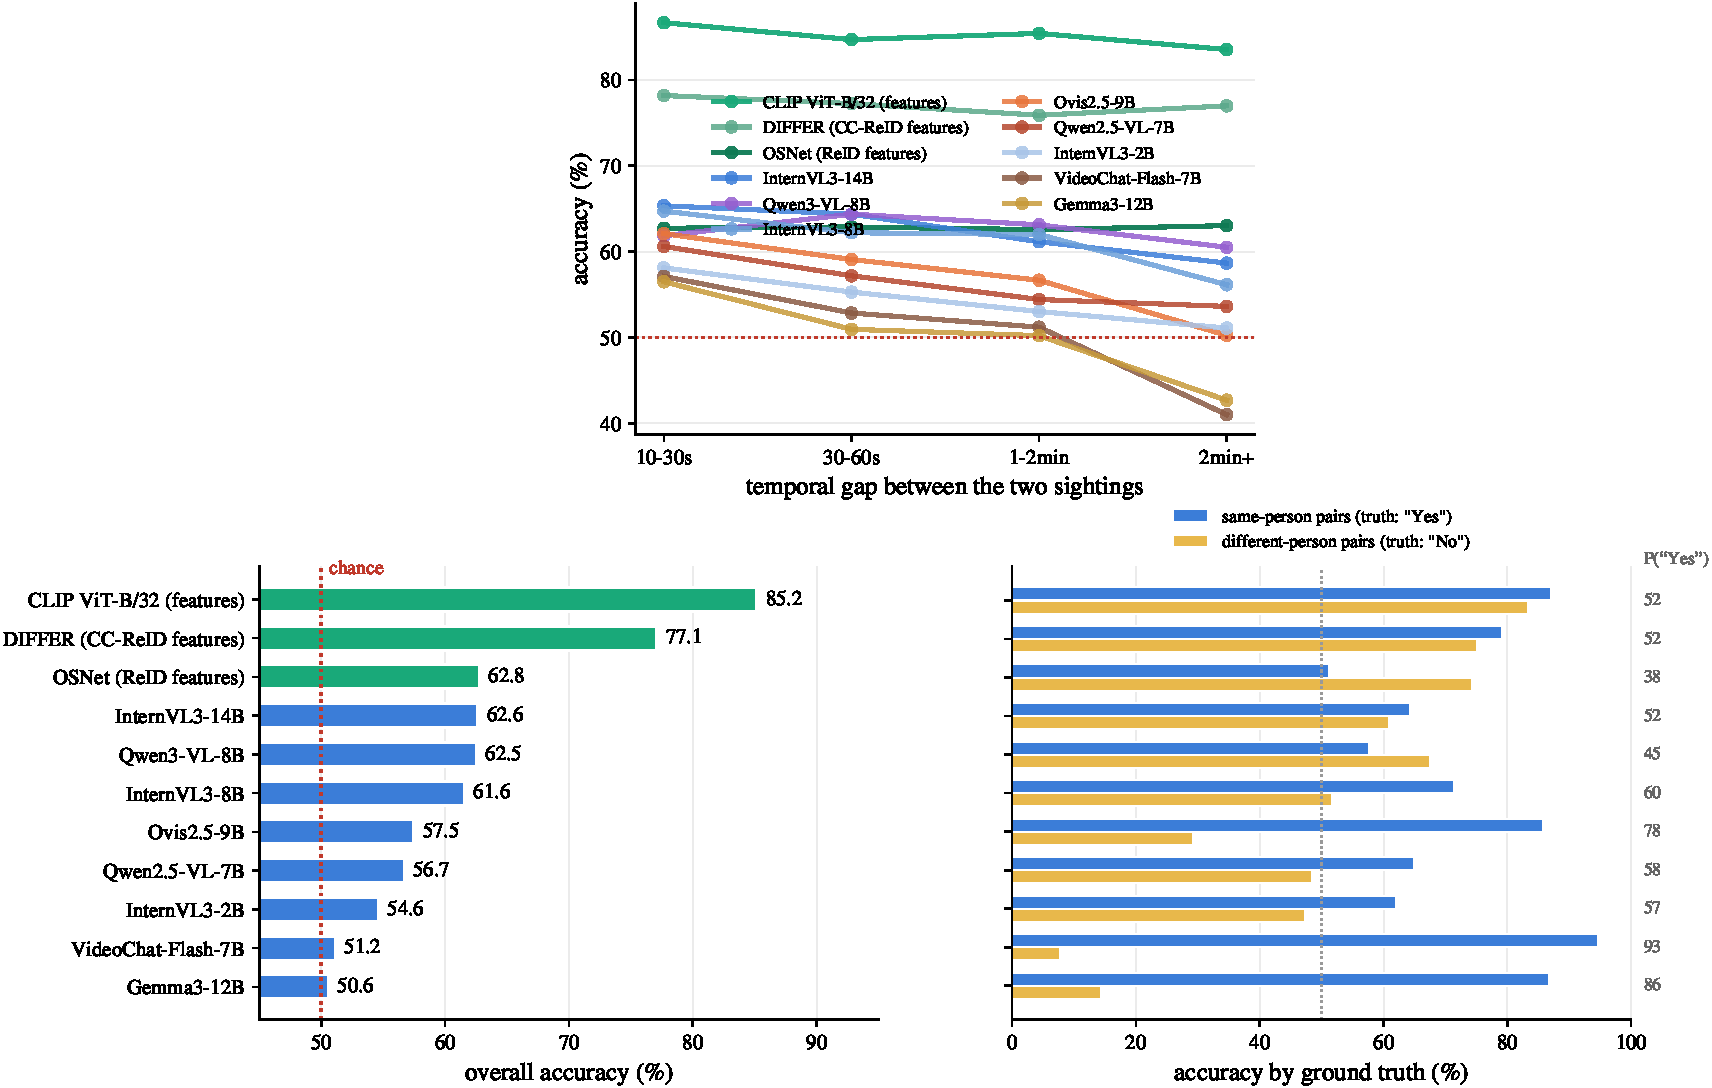
\includegraphics[width=\linewidth]{figures/fig_reid_probe.pdf}
\caption{Same/different-person probe}\label{fig:reidprobe-a}
\end{subfigure}\hfill
\begin{subfigure}[b]{0.375\linewidth}\centering
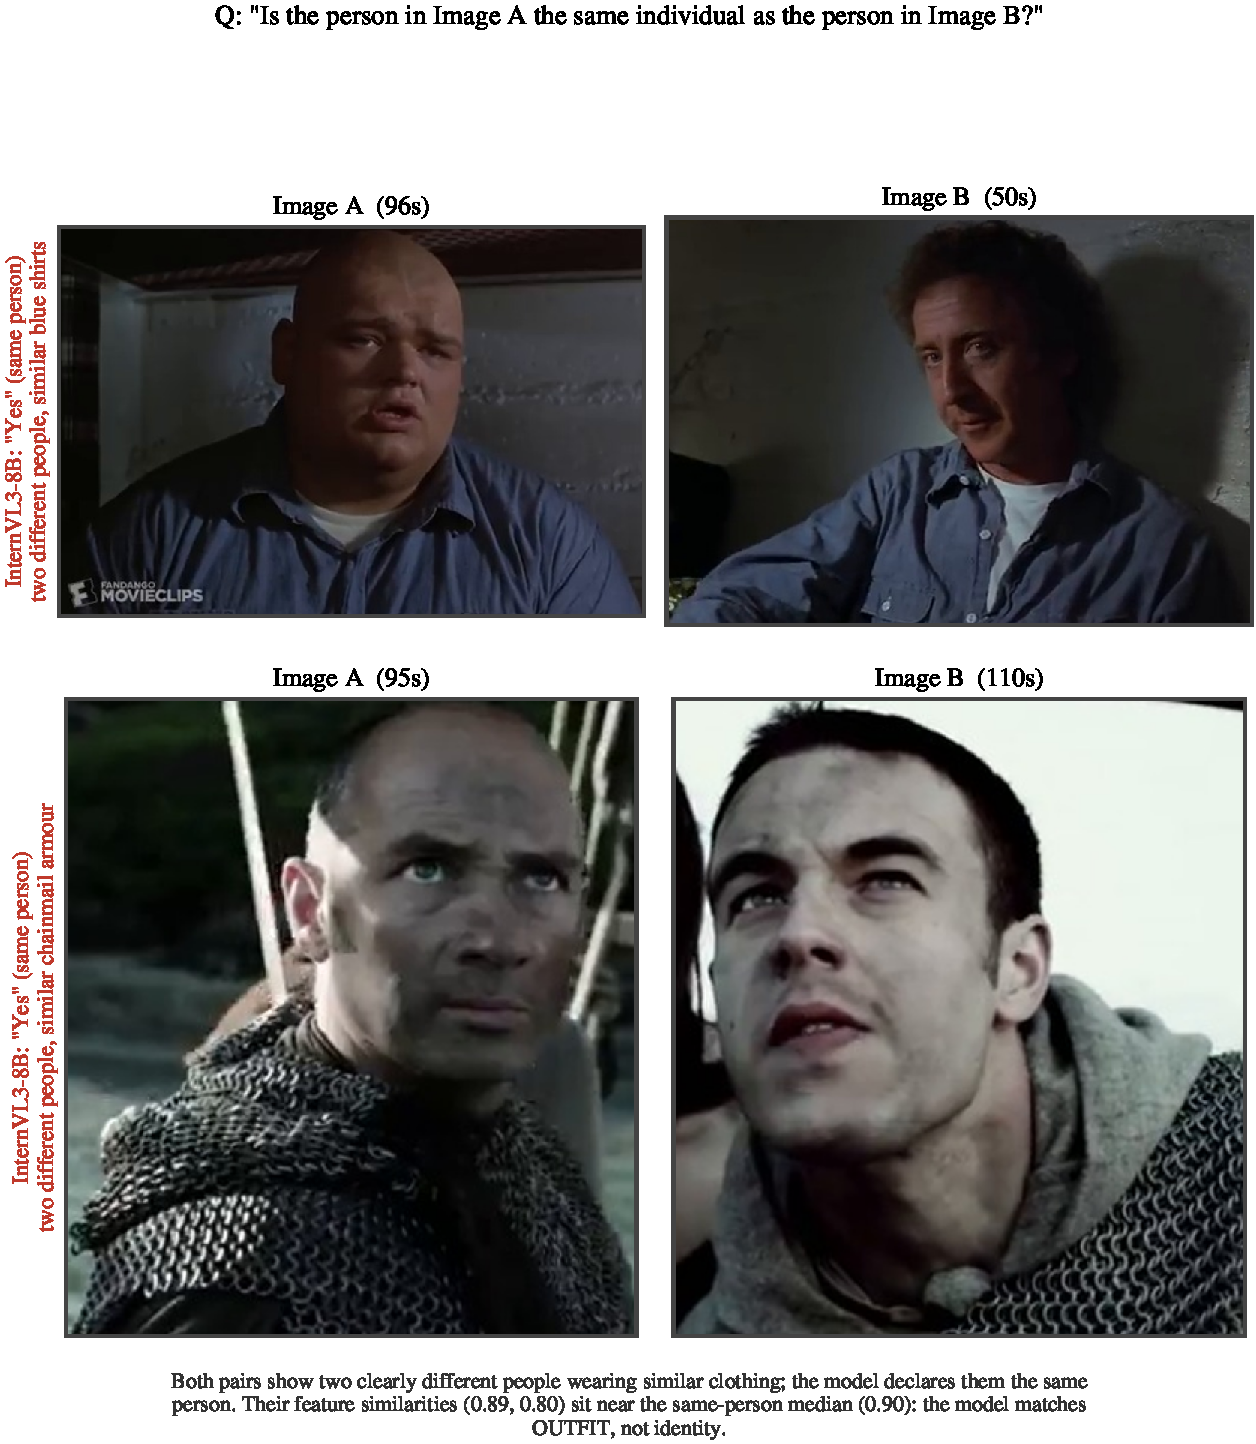
\includegraphics[width=\linewidth]{figures/fig_reid_showcase.pdf}
\caption{Characteristic error}\label{fig:reidprobe-b}
\end{subfigure}
\caption{Models store identity but cannot answer with it. (a) Left, accuracy on 2{,}848 same-or-different-person pairs, where every VLM sits far below a frozen CLIP encoder scored on the identical pairs, and Gemma3-12B is at exactly a coin flip. Right, VLM accuracy decays with the time gap between the two crops while CLIP stays flat. (b) The characteristic error is outfit matching: two different men in the same blue shirt are declared the same person, and the pair's feature similarity (0.89) matches the same-person median (0.90).}
\label{fig:reidprobe}
\end{figure}

\begin{figure}[t]
\centering
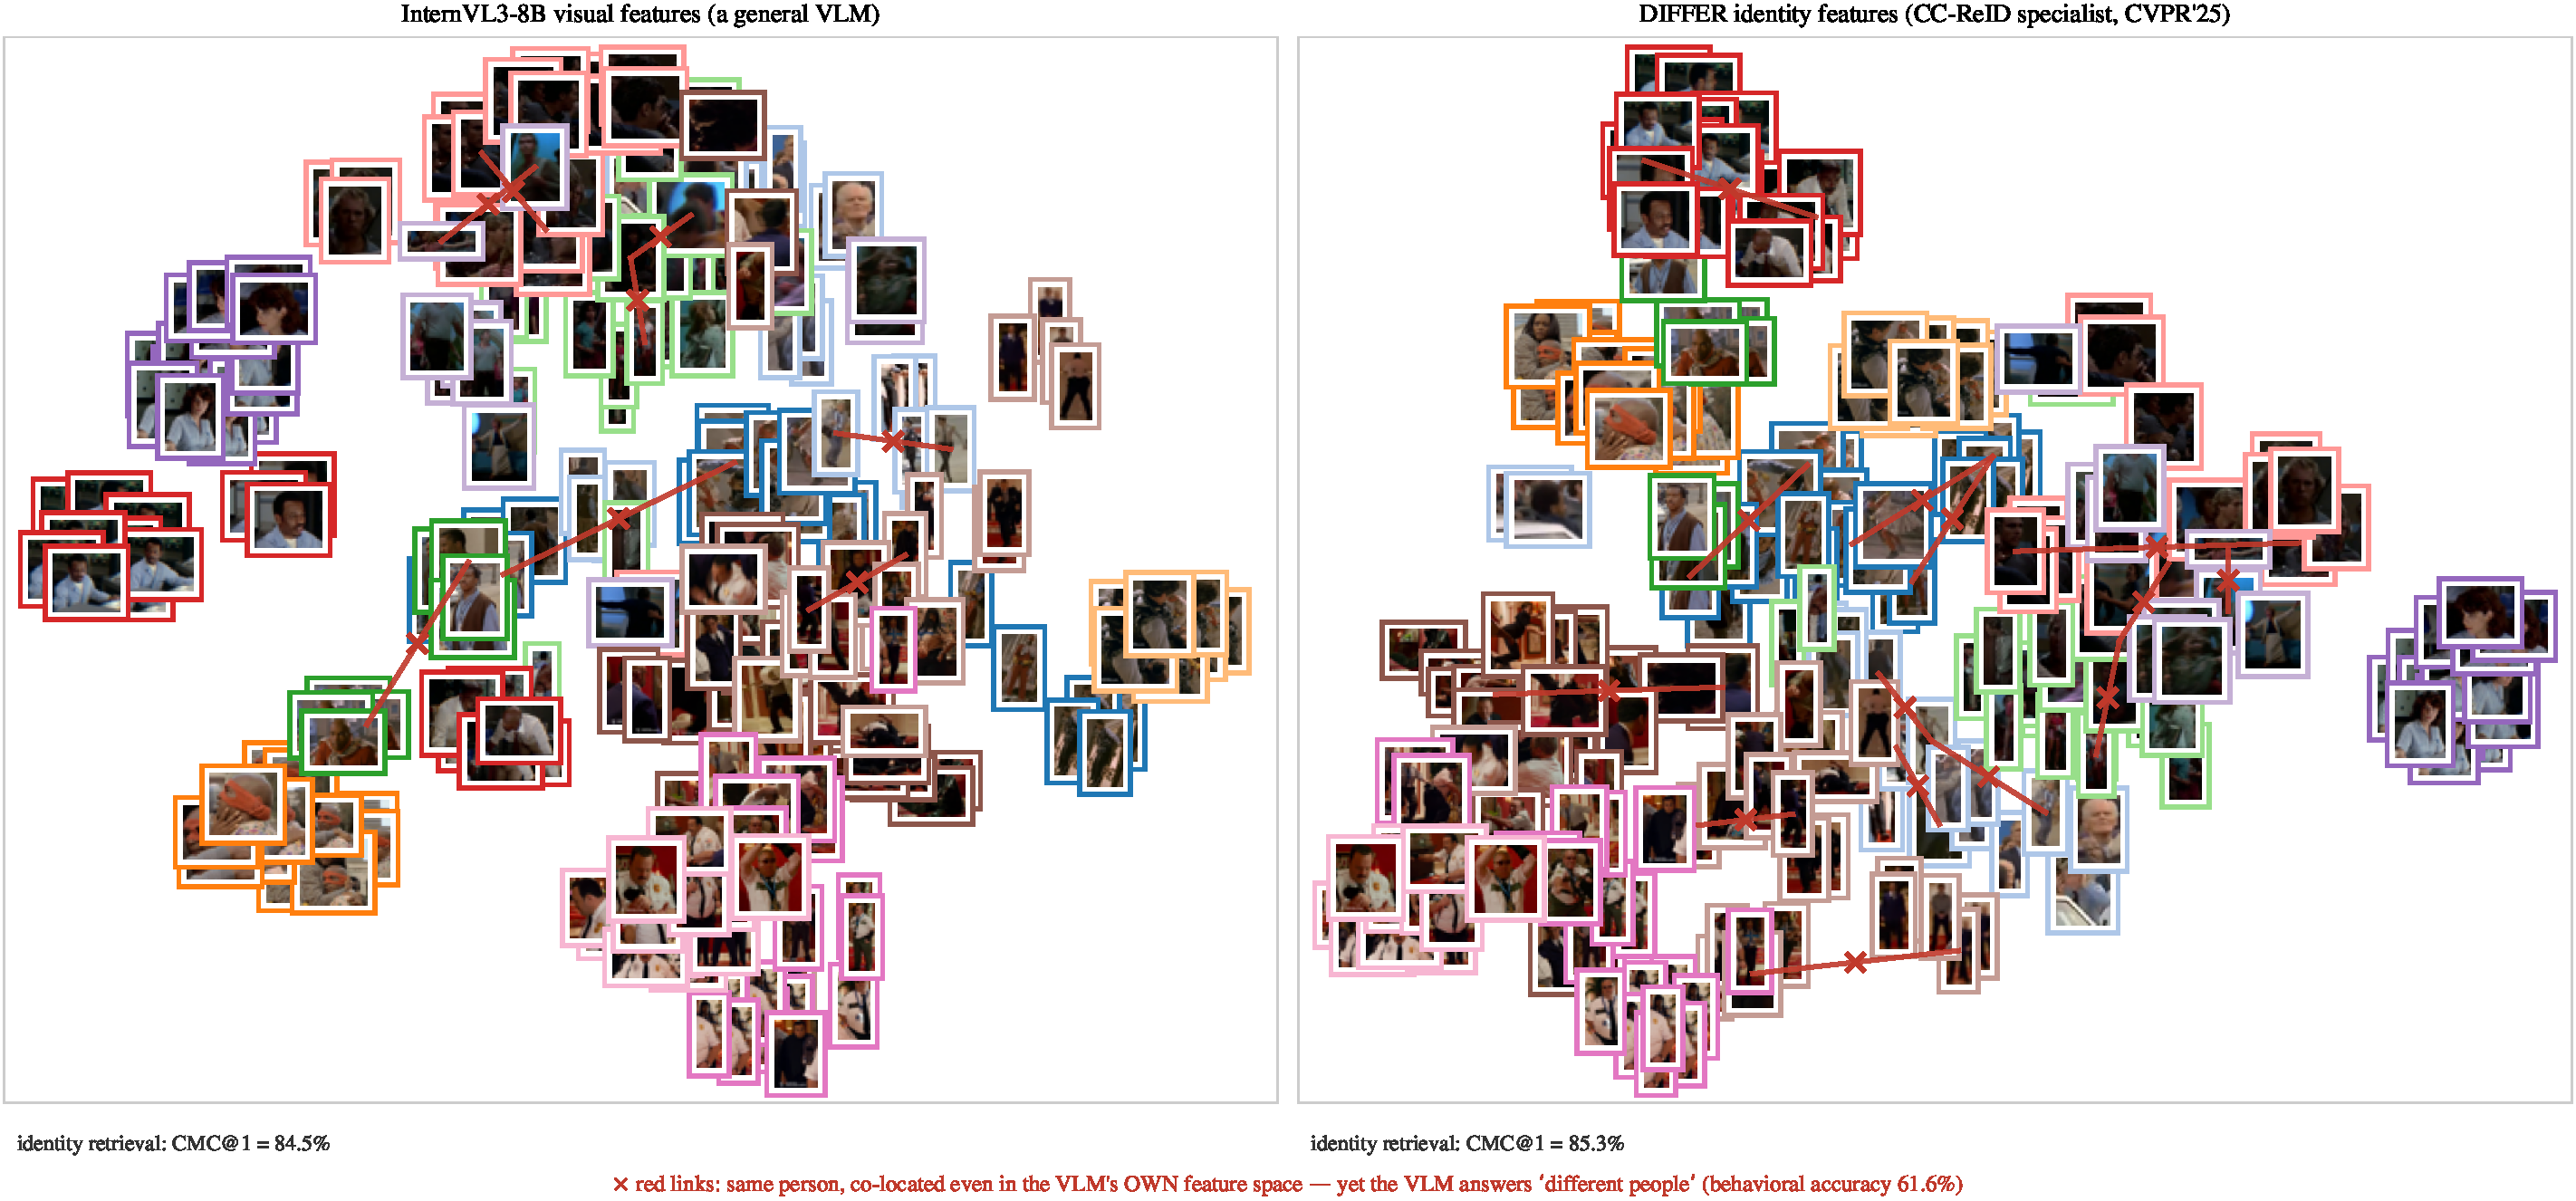
\includegraphics[width=1.0\linewidth]{figures/fig_constellation_differ.pdf}
\caption{t-SNE of InternVL3-8B's own vision features for the person crops of one video, colored by identity. The features separate identities into clean islands (retrieval CMC@1 84.5), and the red links mark behavioral errors, which connect crops that share clothing rather than identity. The model has the information and loses it at answering.}
\label{fig:constellation}
\end{figure}

\subsection{Uniform sampling misses the evidence, causally}
\label{sec:p2}
\textbf{Ground truth for when the evidence is visible.} For each question we localize the moments where the answer can be seen. The strongest leaderboard model receives the question, its correct answer, and 32 densely sampled frames, and only marks when the answer is visible. Verifying a known answer is a far easier task than answering, and 92--94\% of a 50-item human audit confirms the returned windows. This yields evidence windows for 3{,}245 questions. The median window covers 4.4 seconds of a 166-second video, so the task is a needle problem even though the questions never mention time.

\textbf{Uniform grids miss the needle half the time, and every model pays for it.} An 8-frame uniform grid contains no in-window frame for 53\% of questions, and 16 frames still miss 27\% (Figure~\ref{fig:evidence}a). Joining the windows with the cached predictions of all evaluated models shows every model is more accurate when its grid happens to cover the window, by +1.8 to +8.7 points, with the strongest models gaining the most (Figure~\ref{fig:evidence}b). The single flat model is MA-LMM, which Section~\ref{sec:p3} explains: its memory discards the evidence after sampling, so covering it does not help.

\textbf{One frame is causal.} Correlation could reflect confounds, so we intervene on single frames. For a question whose 8-frame grid misses the window, we replace the temporally nearest frame with the window center and rerun the model on the otherwise identical input; for covered questions we do the reverse and move the in-window frame just outside the window. Inserting the evidence frame raises accuracy by +5.0 (InternVL3-14B), +9.7 (Ovis2.5-9B), and +4.3 (Qwen2.5-VL-7B) points, and deleting it costs $-2.7$, $-7.3$, and $-2.7$. Significance uses McNemar's exact test \citep{mcnemar1947}, a paired test that counts only the questions whose correctness flips between the two runs, with $p \le 0.011$ on three of the four tested arms. Figure~\ref{fig:filmstrip} shows one item flipping from wrong to right when a single frame changes. One honest caveat bounds the story: accuracy on covered questions still peaks at 31.9\%, so coverage is necessary but far from sufficient, which motivates the read-out gap of Section~\ref{sec:p1}.

\begin{figure}[t]
\centering
\begin{subfigure}[b]{0.345\linewidth}\centering
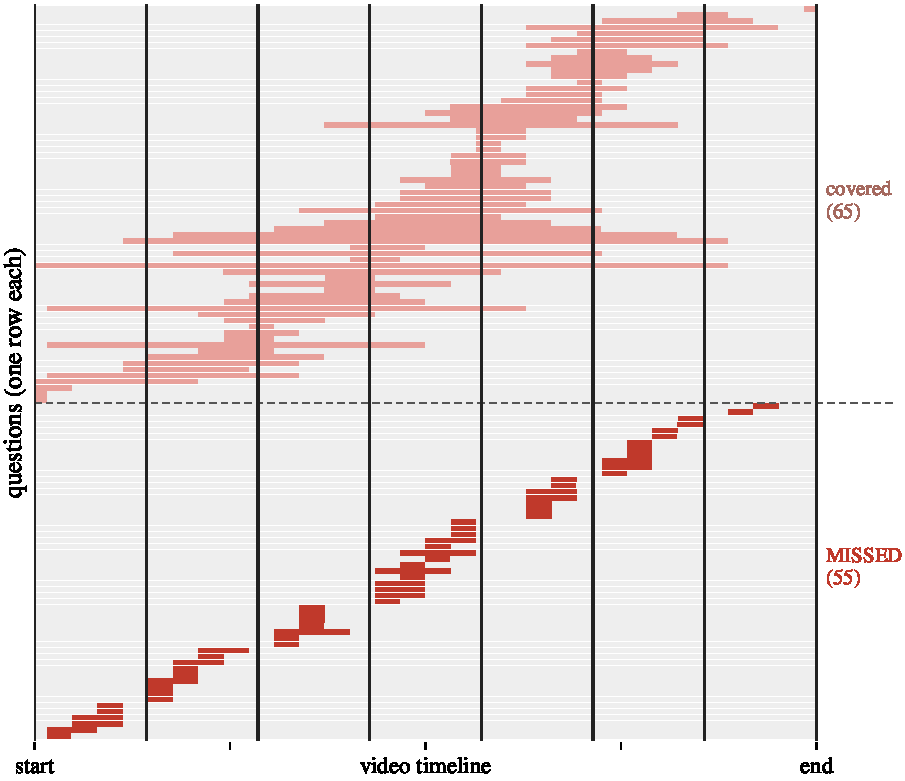
\includegraphics[width=\linewidth]{figures/fig_evidence_barcode.pdf}
\caption{Evidence windows vs.\ uniform grids}\label{fig:evidence-a}
\end{subfigure}\hfill
\begin{subfigure}[b]{0.635\linewidth}\centering
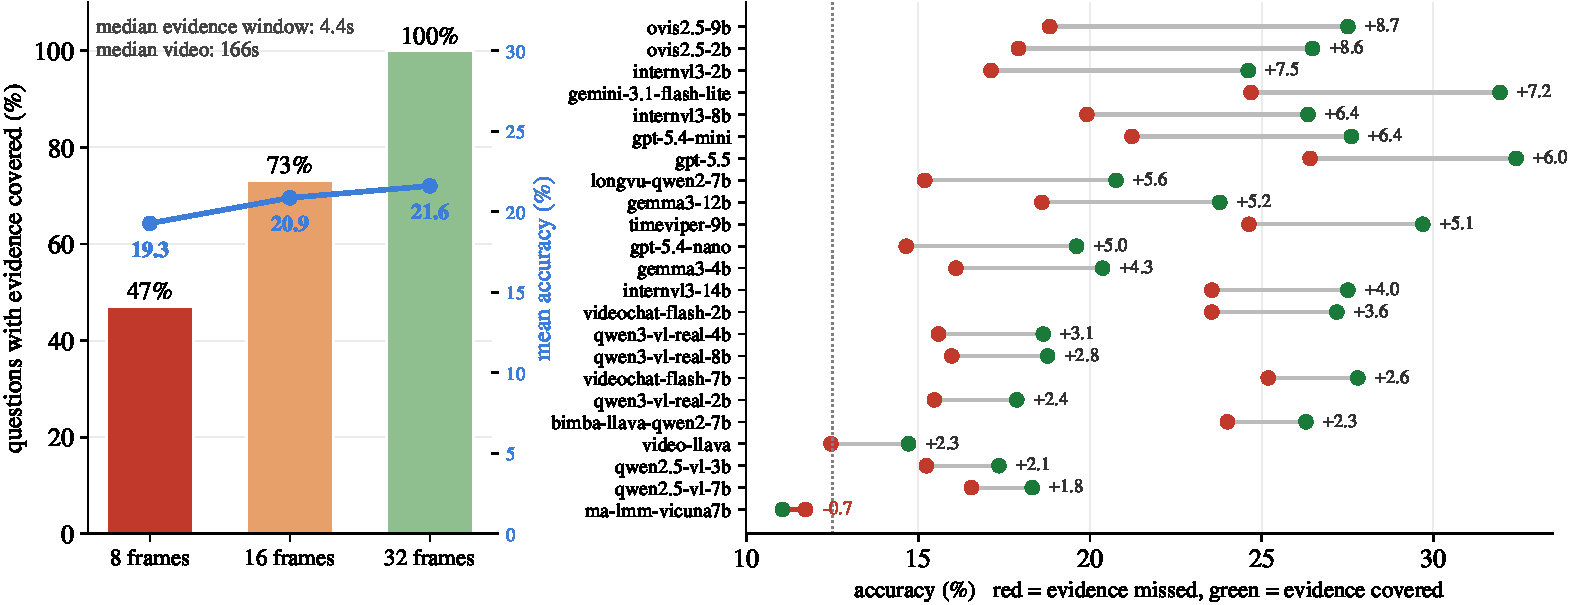
\includegraphics[width=\linewidth]{figures/fig_evidence_coverage.pdf}
\caption{Miss rate and its accuracy cost}\label{fig:evidence-b}
\end{subfigure}
\caption{Uniform sampling misses the evidence. (a) Each row is one question's timeline with its evidence window drawn as a dark band and the uniform sample positions as columns; most windows fall between the columns. (b) Left, the fraction of questions whose evidence window is missed at each uniform budget. Right, per-model accuracy when the grid covers the window against when it misses, where every model gains +1.8 to +8.7 points from coverage and MA-LMM alone is flat.}
\label{fig:evidence}
\end{figure}

\begin{figure}[t]
\centering
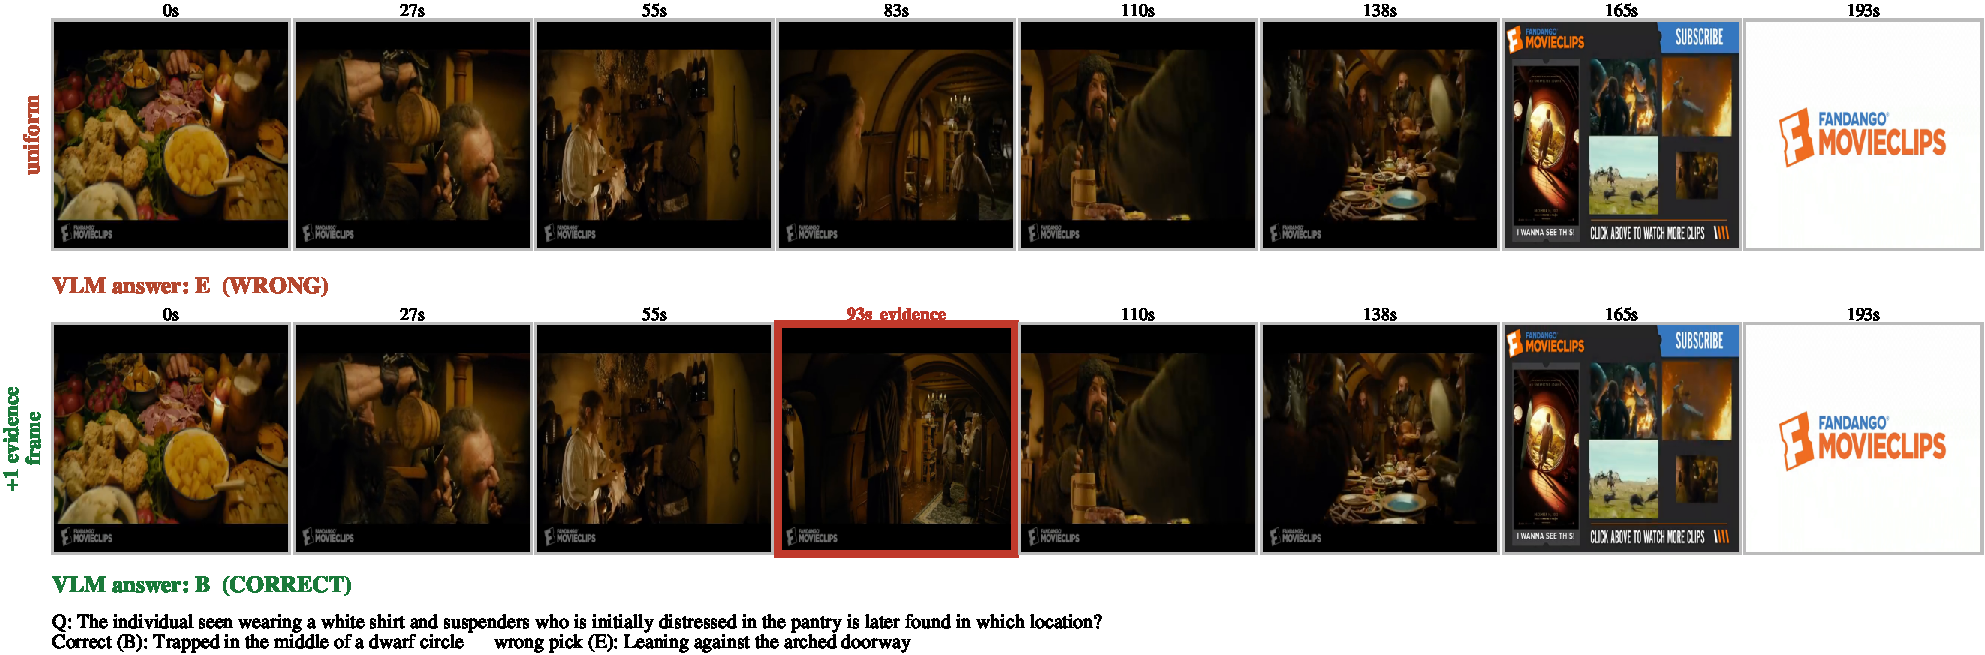
\includegraphics[width=\linewidth]{figures/fig_b3_filmstrip.pdf}
\caption{A single frame is causal. The same question is run twice on identical inputs except one frame: with the evidence frame absent the model answers wrong, and inserting it flips the answer to correct. Aggregated over questions, inserting the evidence frame is worth +4.3 to +9.7 points and deleting it costs 2.7 to 7.3 points (McNemar's exact test, $p \le 0.011$).}
\label{fig:filmstrip}
\end{figure}

\subsection{Memory models lose the evidence in compression, not at retrieval}
\label{sec:p3}
\textbf{Setup.} Five available models compress frames into a token memory: Video-XL-Pro, Video-XL, LongVU, MA-LMM, and VideoChat-Flash, whose hierarchical compression makes it a compression model despite its leaderboard grouping. Two failure stories are possible. Either compression destroys the evidence (a storage failure), or the evidence survives but the model cannot find it when answering (a retrieval failure). We separate them with interventions on a fixed 780-question subset, each model run at its full frame budget, so absolute numbers differ slightly from Table~\ref{tab:leaderboard}. A \emph{hint} appends to the prompt exactly when the evidence occurs (e.g., \emph{the relevant moment is around 62--66 seconds}), which repairs retrieval but adds no pixels. \emph{Evidence-only} instead feeds the model only its evidence window, which repairs storage by making compression unnecessary. Controls bound both: a wrong hint, a random window of the same length, and a variant that guarantees one evidence frame inside the usual uniform grid.

\textbf{Hints do nothing, evidence-only splits the field.} Telling every model when to look moves accuracy by at most $+0.9$ points, so retrieval is not the bottleneck for any model (Table~\ref{tab:interventions}). Feeding only the evidence lifts LongVU by $+9.8$ and VideoChat-Flash by $+5.9$, so for these two the information was destroyed before answering, a storage failure. The Video-XL family gains only about $+3$, and its guaranteed-frame control gains nothing, so its failure is not about which frames enter but about reading them, and MA-LMM stays at chance even when handed the exact evidence, so no input strategy can rescue it. Sweeping Video-XL's compression ratio from $2\times$ to $32\times$ costs only 2 points (17.0 to 15.0), so memory capacity is not the binding constraint either.

\textbf{Classifying every question.} Combining the three runs classifies each question per model (Figure~\ref{fig:p3matrix}): answered at baseline; retrieval-bound if the hint alone fixes it; storage-bound if only evidence-only fixes it; perception-bound if the model fails even on the evidence alone. Perception-bound failures dominate every model at 61 to 78\% of questions, storage-bound failures are twice as common for LongVU (13\%) and VideoChat-Flash (12\%) as for the Video-XL family (5--6\%), and retrieval-bound failures are negligible (1--3\%) everywhere except MA-LMM (5\%). Since single 8-way runs carry guess noise near the 12.5\% chance rate, we read the ordering of the bars rather than any single cell, and the controls above bound the noise.

\textbf{Watching the memory decide.} We instrument each model's compression step with forward hooks and record how much of each input frame survives into the final memory, using each model's native mechanism: MA-LMM's memory-bank merge tree \citep{malmm}, LongVU's frame-selection masks \citep{longvu}, Video-XL-Pro's token-keep decisions \citep{videoxlpro}, and VideoChat-Flash's token-merging mass \citep{videochatflash,tome}. No model's compression favors the frames that carry the answer, with an evidence-minus-background retention gap of only $+0.016$ to $+0.019$, so these memories are evidence-blind, and MA-LMM's gap is negative ($-0.021$) because its bank retains almost exclusively the end of the video (Figure~\ref{fig:p3matrix}b). Figure~\ref{fig:album} makes this concrete: on one video the mid-video evidence retains 4.5\% of the memory mass while the closing frames retain 57\%, and those closing frames are the uploader's outro cards. This closes the loop with Section~\ref{sec:coverage}: compression models fail because their token budget is spent blind to the query, which is exactly what the query-conditioned allocation of Section~\ref{sec:method} targets.

\begin{table}[t]
\centering
\caption{Interventions on the five compression models (accuracy \%, fixed 780-question subset, each model at its full frame budget). A when-hint repairs retrieval without adding pixels and moves no model; feeding only the evidence window repairs storage and splits the field. Controls: a random window of the same length scores 14.9 on Video-XL-Pro, and guaranteeing one evidence frame inside the uniform grid leaves it at 20.0.}
\label{tab:interventions}
\small
\begin{tabular}{@{}lcccl@{}}
\toprule
Model & Baseline & When-hint & Evidence-only & Reading \\
\midrule
LongVU & 18.1 & 19.0 & \textbf{27.9} ($+9.8$) & storage: compression destroys evidence \\
VideoChat-Flash & 26.0 & 24.6 & \textbf{31.9} ($+5.9$) & storage: compression destroys evidence \\
Video-XL-Pro & 20.0 & 19.8 & 23.1 ($+3.1$) & perception: fails even on clean evidence \\
Video-XL & 19.4 & 19.6 & 22.3 ($+2.9$) & perception: fails even on clean evidence \\
MA-LMM & 11.1 & 11.9 & 13.2 ($+2.1$) & at chance even on evidence \\
\bottomrule
\end{tabular}
\end{table}

\begin{figure}[t]
\centering
\begin{subfigure}[b]{0.50\linewidth}\centering
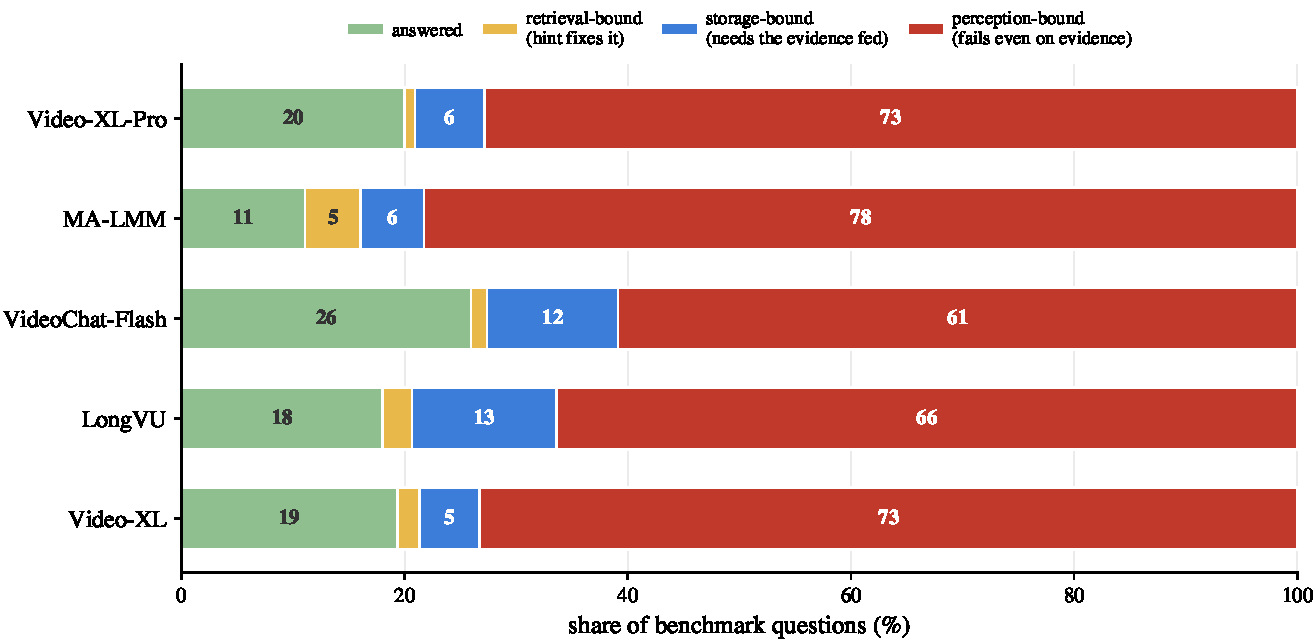
\includegraphics[width=\linewidth]{figures/fig_decision_matrix.pdf}
\caption{Per-question failure classification}\label{fig:p3matrix-a}
\end{subfigure}\hfill
\begin{subfigure}[b]{0.48\linewidth}\centering
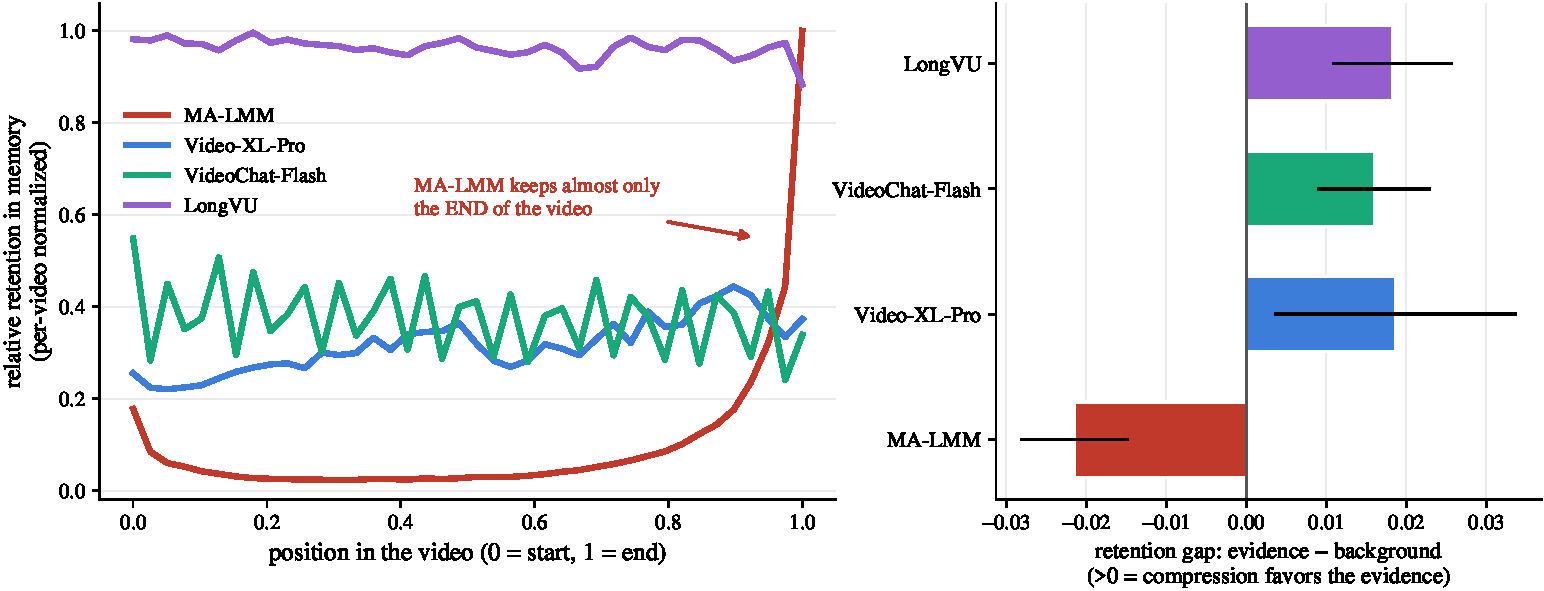
\includegraphics[width=\linewidth]{figures/fig_memory_survival.pdf}
\caption{What the memory retains}\label{fig:p3matrix-b}
\end{subfigure}
\caption{Storage, not retrieval. (a) Every question classified per model from the intervention runs. Perception-bound failures dominate (61--78\%), storage-bound failures are twice as common for the two models whose compression destroys evidence, and pure retrieval failures are negligible. (b) Left, token retention against position in the video, where MA-LMM keeps almost only the ending. Right, the evidence-minus-background retention gap per model, which is near zero everywhere and negative for MA-LMM, so no memory favors the frames that carry the answer.}
\label{fig:p3matrix}
\end{figure}

\begin{figure}[t]
\centering
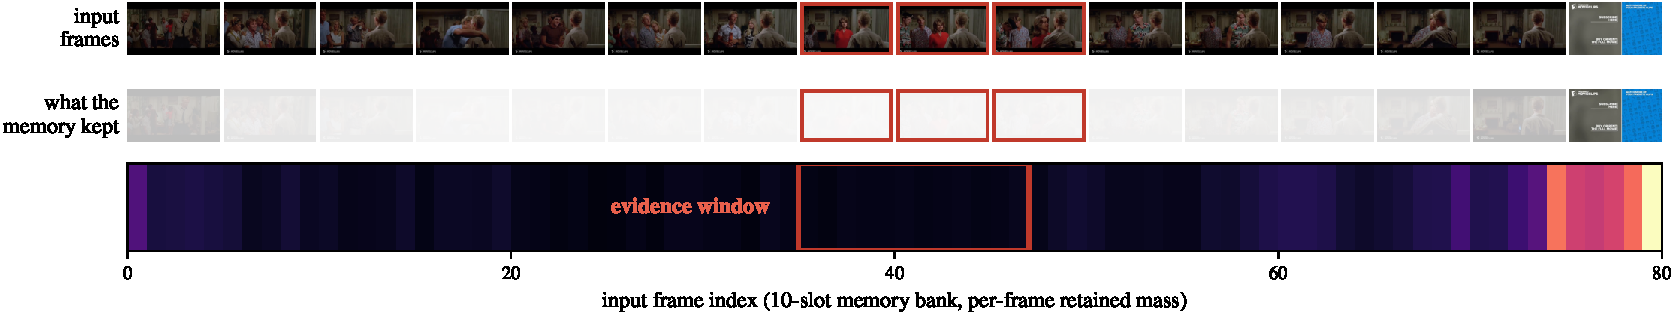
\includegraphics[width=\linewidth]{figures/fig_malmm_album.pdf}
\caption{What MA-LMM's memory remembers, on one benchmark video. Top, the input frames; middle, the same frames faded by how little mass the 10-slot memory bank retains for them; bottom, per-frame retained mass. The mid-video evidence window (red) retains 4.5\% of the memory mass while the closing frames retain 57\%, and the closing frames are the uploader's outro cards.}
\label{fig:album}
\end{figure}

\textbf{One failure chain.} The three diagnostics compose. The frames that carry the answer usually never enter the model, and single frames are causally worth 5 to 10 points (Section~\ref{sec:p2}). When the right frames do enter, identity is demonstrably present in the visual features but is lost at answering, collapsing to outfit matching (Section~\ref{sec:p1}). And the compression architectures built to widen coverage spend their token budget blind to the query, so they destroy the same evidence sampling misses (Section~\ref{sec:p3}). The dominance of perception-bound failures, 61 to 78\% even with clean evidence, explains why every input-side fix in Section~\ref{sec:coverage} saturates near two points: better frames cannot repair a read-out that discards what the features already know.

\section{Toward Closing the Gap}
\label{sec:method}
The diagnosis implies a mechanism. Coverage requires compression and compression destroys the fidelity this task needs, so the token budget should be spent non-uniformly and conditioned on the referent and question. We test this as an inference-time change to Video-XL-Pro, keeping its 128-token budget but allocating dense frames around moments a CLIP score marks as query-relevant. On a matched 463-question subset this raises accuracy from 14.0\% to 16.0\%, a 2.0-point gain with no training. The gain motivates a learned importance head that keeps referent tokens dense while compressing the rest, trained on 16{,}808 held-out videos with zero benchmark overlap. We report the training-free result here and leave the learned method to future work, so the benchmark remains the contribution.

\section{Conclusion}
\bench{} measures a skill that long video systems are assumed to have and do not, namely following one identity through a long video and reading fine-grained attributes about it. The benchmark is debiased against language priors, richly tagged, and unsaturated. The analysis rejects the identity-confusion reading, since dedicated re-identification pipelines do not help and identity-confusion proxies do not predict difficulty. The limit is the joint allocation of temporal coverage and per-frame fidelity that current architectures trade against each other, and temporal tracking skills define the frontier new methods must attack.

\subsubsection*{Reproducibility statement}
Every evaluation runs zero-shot with a shared prompt, parser, and sampler. We release per-model predictions for every question, the analysis code that produces every figure and table, and the shortcut audits. Thirty source videos that the local decoding stack could not read are excluded from every model, and their identifiers are released so the exclusion is reproducible. The videos come from public collections and are referenced by identifier. The method of Section~\ref{sec:method} is trained only on a disjoint video set with a released overlap audit.

\newpage
\bibliography{references}
\bibliographystyle{iclr2026_conference}

\newpage
\appendix
\section{Extended composition}
\label{app:composition}
\bench{} is designed to spread questions across perceptual skills and re-identification challenges rather than concentrate on any single type. Table~\ref{tab:composition} lists the capability and challenge axes, and the referral axis records how each question names its referent, with 1001 mixed-reference, 906 appearance-reference, 901 activity-reference, 477 location-reference, and 375 environment-reference questions. Referents are people in 74\% of questions and animals in 26\%, which keeps the benchmark from collapsing to face recognition. The difficulty axis is assigned at construction time and later audited against measured accuracy in Appendix~\ref{app:diffcal}.

Figure~\ref{fig:vstats} shows the video and question distributions. The median video runs 3.2 minutes with 53 shot cuts, the median maximum concurrent-person count is 2, and the median option length is 7 words. The high cut rate is the reason cross-shot identity persistence is intrinsic to the domain, since a referent introduced in one shot is typically re-shown after several intervening cuts. Option lengths are tightly distributed around 7 words, which limits the length cue that a model could exploit, and the residual longest-option-is-correct rate of 16.8\% reported in the main text reflects this control. Every distribution is computed over the full released set of \numq{} questions and \numv{} videos. The challenge counts are deliberately uneven, since the axis mirrors how often each re-identification event occurs in movie footage rather than an imposed uniform prior. Rare types such as role or position swap at 11 questions and occlusion recovery at 26 questions are reported as their own slices rather than merged into neighbors, which keeps a hard slice from being diluted, at the cost of wider bootstrap intervals on those slices.
\begin{figure}[h]
\centering
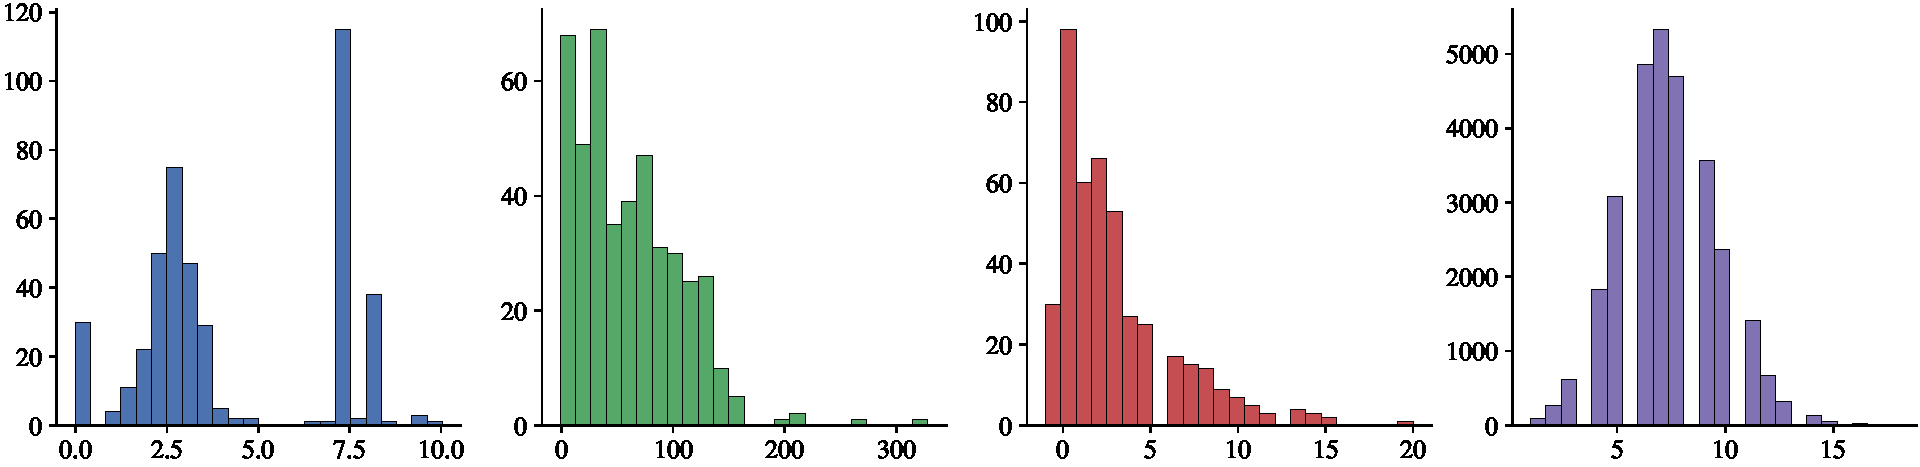
\includegraphics[width=0.9\linewidth]{figures/fig_video_stats.pdf}
\caption{Video and question statistics, namely duration, shot cuts, concurrent people, and option length.}
\label{fig:vstats}
\end{figure}


Table~\ref{tab:composition} reports the composition of the benchmark along the capability
and re-identification challenge axes; Table~\ref{tab:axis-defs} defines every value on both
axes so a reader can reproduce the tagging. Tags are assigned from the dense per-video
annotation and verified in the same retagging pass that produced the frozen release.

\begin{table}[t]
\centering
\small
\renewcommand{\arraystretch}{1.15}
\caption{\textbf{Metadata axis definitions.} Every question carries exactly one
capability tag (the perceptual attribute of the referent the question probes) and one
re-identification challenge tag (the kind of identity tracking the question requires,
ordered from least to most temporal structure).}
\label{tab:axis-defs}
\begin{tabularx}{\textwidth}{@{}l X@{}}
\toprule
\multicolumn{2}{@{}l}{\textsc{Capability axis}} \\
\midrule
Appearance    & What the referent looks like, including clothing, color, accessories, and physical traits. \\
Activity      & The action the referent performs, such as walking, sitting, throwing, or speaking. \\
Location      & Where the referent is, including the room, setting, or place within the scene. \\
Interaction   & How the referent engages another person or object, such as handing, holding, or facing. \\
Object state  & The state or attribute of an object the referent uses or stands near, such as open, lit, or empty. \\
\midrule
\multicolumn{2}{@{}l}{\textsc{Re-identification challenge axis}} \\
\midrule
1.\; Single-shot reference         & The referent is introduced and asked about within one continuous shot, so re-identification is minimal. \\
2.\; Cross-scene re-identification & The referent is introduced in one scene and asked about after a cut to a different scene. \\
3.\; Long-term tracking            & The referent must be followed across a long temporal gap between introduction and query. \\
4.\; Multi-hop tracking            & The referent is reached through a chain of references, e.g., \emph{the person who spoke to the man in red}. \\
5.\; Appearance change             & The referent changes clothing or accessories between introduction and query, so appearance alone is unreliable. \\
6.\; Action sequence               & The answer depends on an ordered sequence of actions the referent performs over time. \\
7.\; Spatial relationship          & The answer depends on the spatial relation between the referent and another person or object. \\
8.\; Disambiguation (similar)      & Several visually similar identities are present and the referent must be distinguished from its lookalikes. \\
9.\; Occlusion recovery            & The referent is occluded or leaves the frame and must be re-found when it reappears. \\
10.\; Role/position swap           & Two identities exchange roles or screen positions and must be kept distinct through the swap. \\
\bottomrule
\end{tabularx}
\end{table}

\section{Leaderboard in chart form}
\label{app:leaderboard}
Figure~\ref{fig:leaderboardchart} presents the leaderboard of Table~\ref{tab:leaderboard} as grouped horizontal bars, which makes the three-way split visible at a glance. GPT-5.5 leads at 29.5\%, the full-fidelity open models occupy a broad middle band, and the token-compression models cluster at the bottom despite reading far more frames. The bars also show how tightly the field packs between 16\% and 26\%, which is the reason the benchmark discriminates methods rather than saturating. Each bar uses the same per-model frame budget as Table~\ref{tab:leaderboard}, so bar length is directly comparable to the tabulated accuracy. Coloring by family makes the within-family spread visible and shows that no single family owns the middle band.




\begin{figure}[b]
\centering
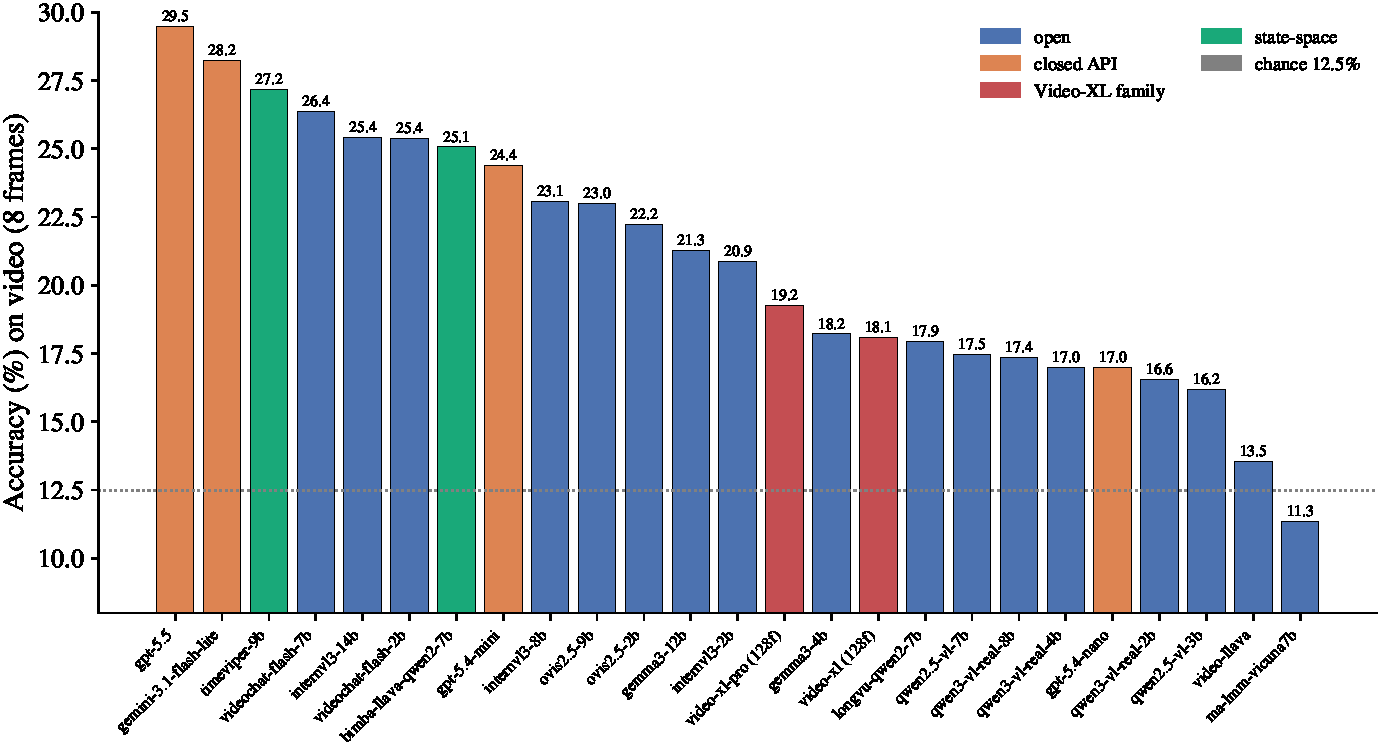
\includegraphics[width=0.82\linewidth]{figures/fig_leaderboard.pdf}
\caption{\bench{} leaderboard as grouped bars, colored by model family. Chance is 12.5\%.}
\label{fig:leaderboardchart}
\end{figure}

\section{Difficulty calibration and per-slice accuracy}
\label{app:diffcal}
We compute every per-slice number as the mean accuracy over all \nummodels{} evaluated models, which smooths idiosyncrasies of any single model and reflects the difficulty the benchmark poses to the field. Assigned difficulty labels track measured accuracy weakly and non-monotonically, at 20.6\% easy, 17.5\% medium, and 19.2\% hard, shown in Figure~\ref{fig:diffcal}. The non-monotonicity means the labels are useful for coarse stratification but not for fine ranking, so every difficulty-conditioned analysis in the main text uses measured consensus difficulty, defined as the number of models that answer a question correctly, rather than the assigned label.

Figure~\ref{fig:capslice} breaks accuracy down by probed capability. The five capabilities span a narrow band, which shows that difficulty is not driven by one capability but by the re-identification demand that cuts across all of them. Figure~\ref{fig:posbias} shows the predicted-letter distribution per model against the balanced correct-answer distribution. Most models stay close to the uniform 12.5\% per letter, but several token-compression models over-predict early letters when uncertain, which is visible as a warm left edge and which the committee filtering in the main text does not remove because it is a model behavior rather than a data artifact. We release the full letter histograms so that any position-driven inflation can be audited per model. Figure~\ref{fig:agree} shows the pairwise correctness correlation between models, which averages $\phi=0.24$ and reaches 0.54, so models tend to fail on the same questions rather than independently, and the two compression models with the strongest letter bias sit apart from the main cluster. Averaging every per-slice number over \nummodels{} models trades per-model resolution for a stable field-level estimate, so a slice describes the difficulty the benchmark poses to the field rather than any one system. Slices with fewer than 30 questions carry wide bootstrap intervals and are read as directional only.
\begin{figure}[tp]
\centering
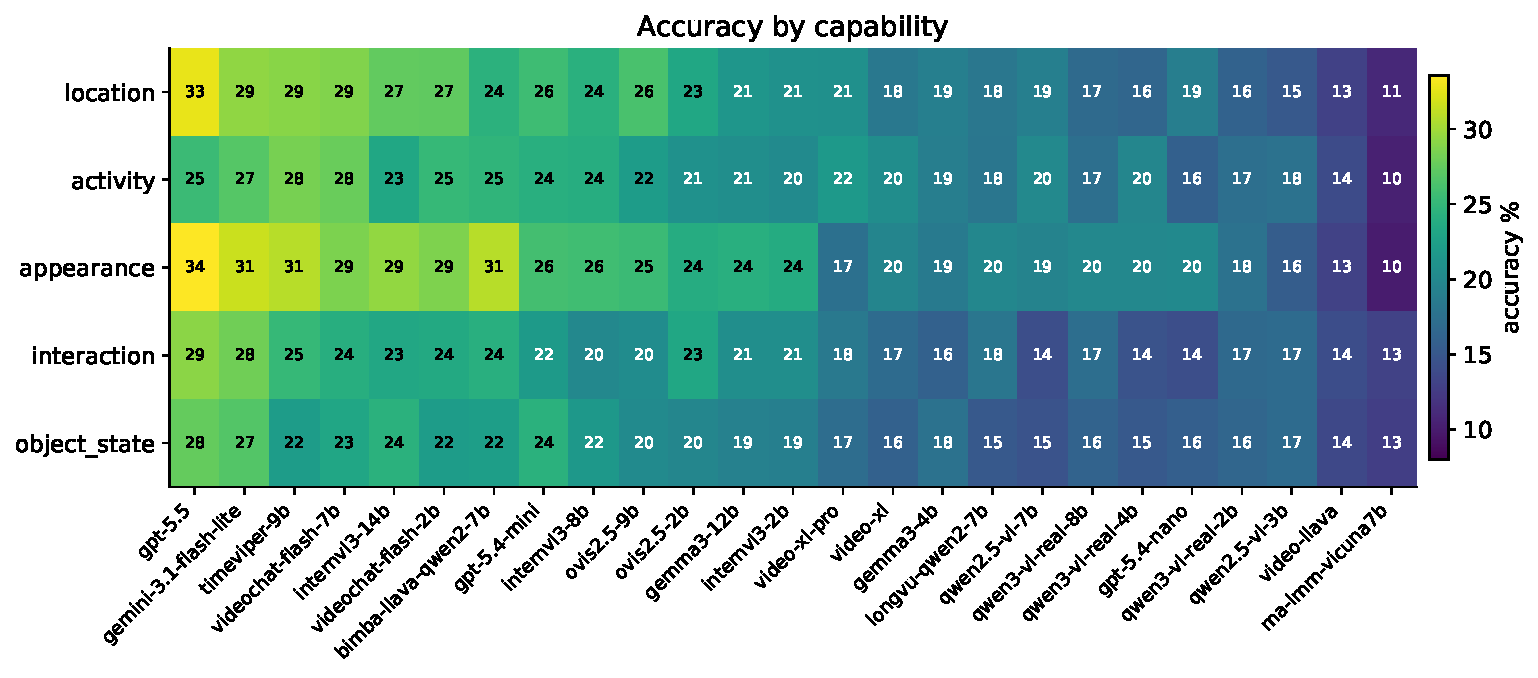
\includegraphics[width=\linewidth]{figures/slice_capability.pdf}
\caption{Accuracy of each model by probed capability. The five capabilities span a narrow band, so difficulty is not driven by any single capability but by the re-identification demand cutting across all of them.}
\label{fig:capslice}
\end{figure}
\begin{figure}[tp]
\centering
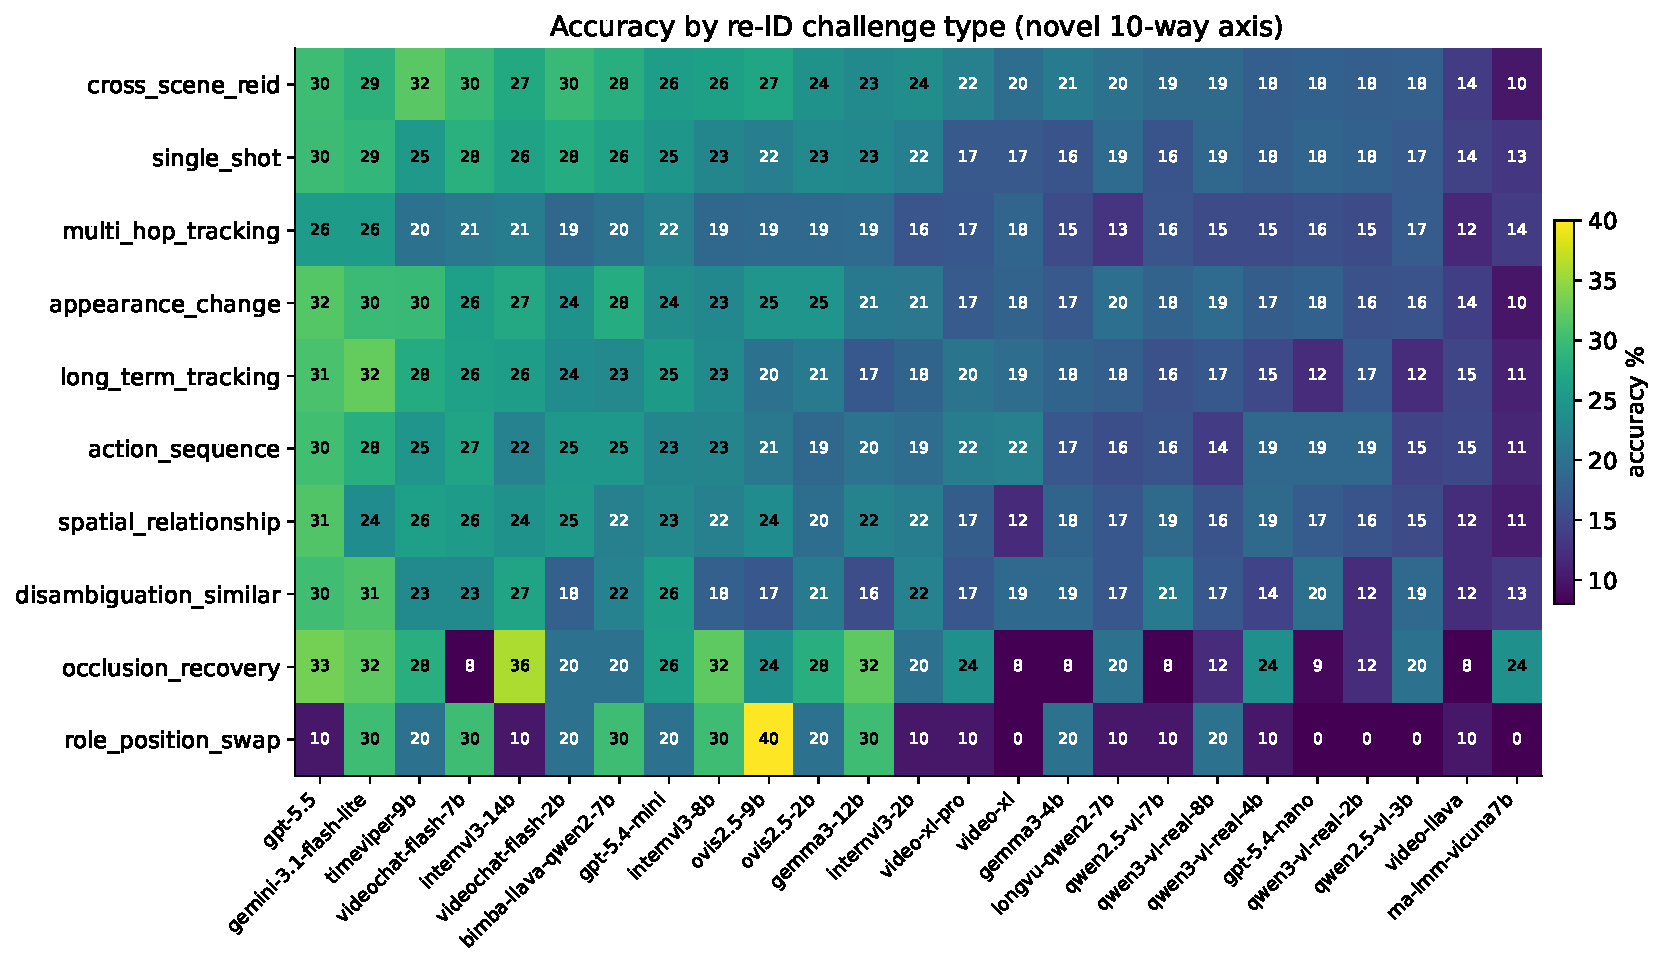
\includegraphics[width=\linewidth]{figures/slice_reid_canonical.pdf}
\caption{Accuracy of each model on each challenge type. Temporal tracking skills, namely role swaps, multi-hop tracking, and long-term tracking, are hardest across every model, and single-scene appearance types are easiest. This is the full per-model heatmap for the hierarchy summarized in Section~\ref{sec:skills}.}
\label{fig:reidslice}
\end{figure}
\begin{figure}[b]
\centering
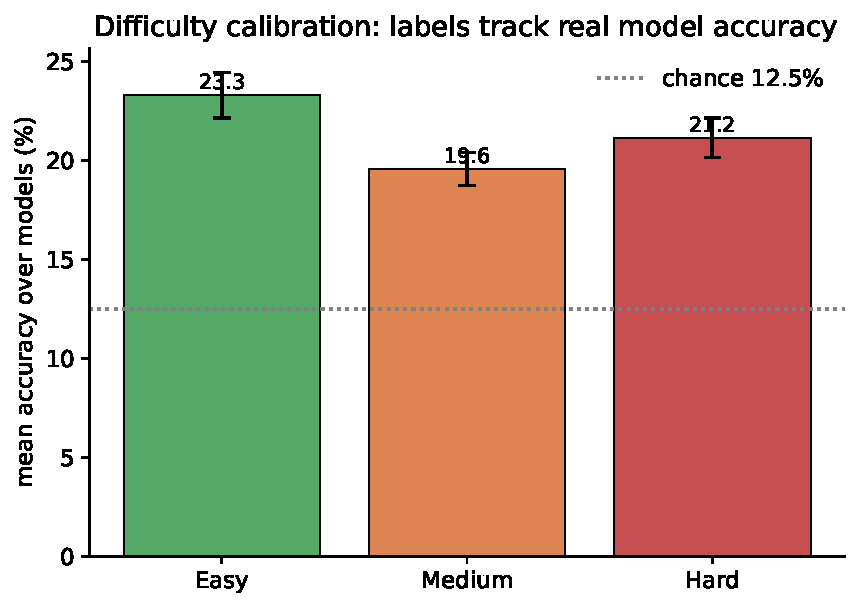
\includegraphics[width=0.5\linewidth]{figures/fig_difficulty_calibration.pdf}
\caption{Mean accuracy over models by assigned difficulty against a \chance{} chance level. The relation to the assigned label is weak and non-monotonic, which motivates using measured consensus difficulty instead.}
\label{fig:diffcal}
\end{figure}
\begin{figure}[t]
\centering
\begin{subfigure}{0.99\linewidth}\centering
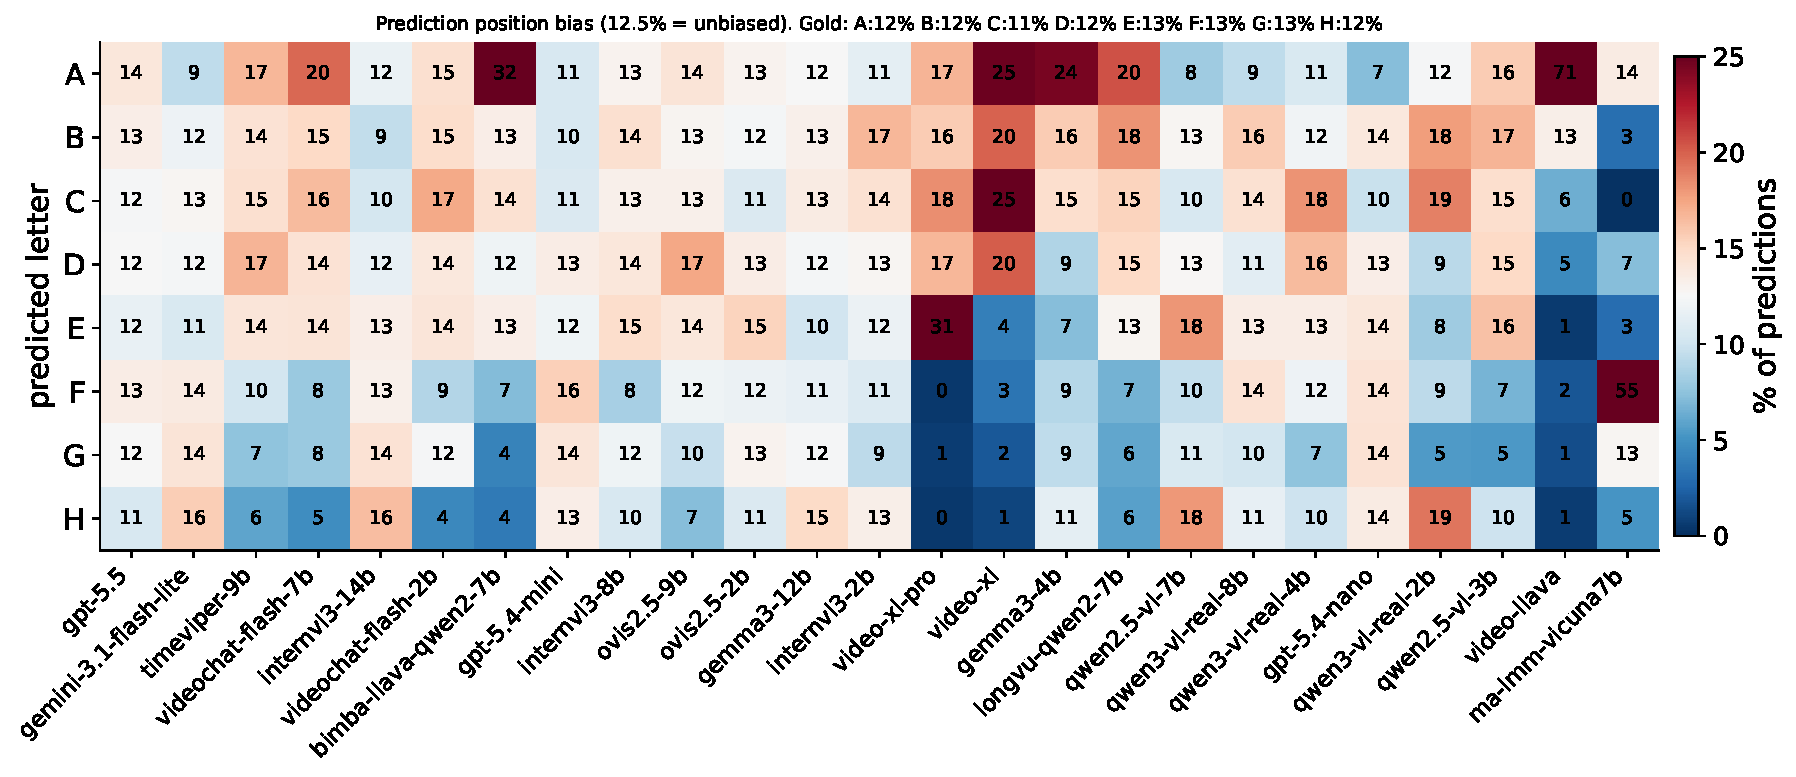
\includegraphics[width=\linewidth]{figures/fig_position_bias.pdf}
\caption{Position bias}\label{fig:posbias}
\end{subfigure}\\[4pt]
\begin{subfigure}{0.72\linewidth}\centering
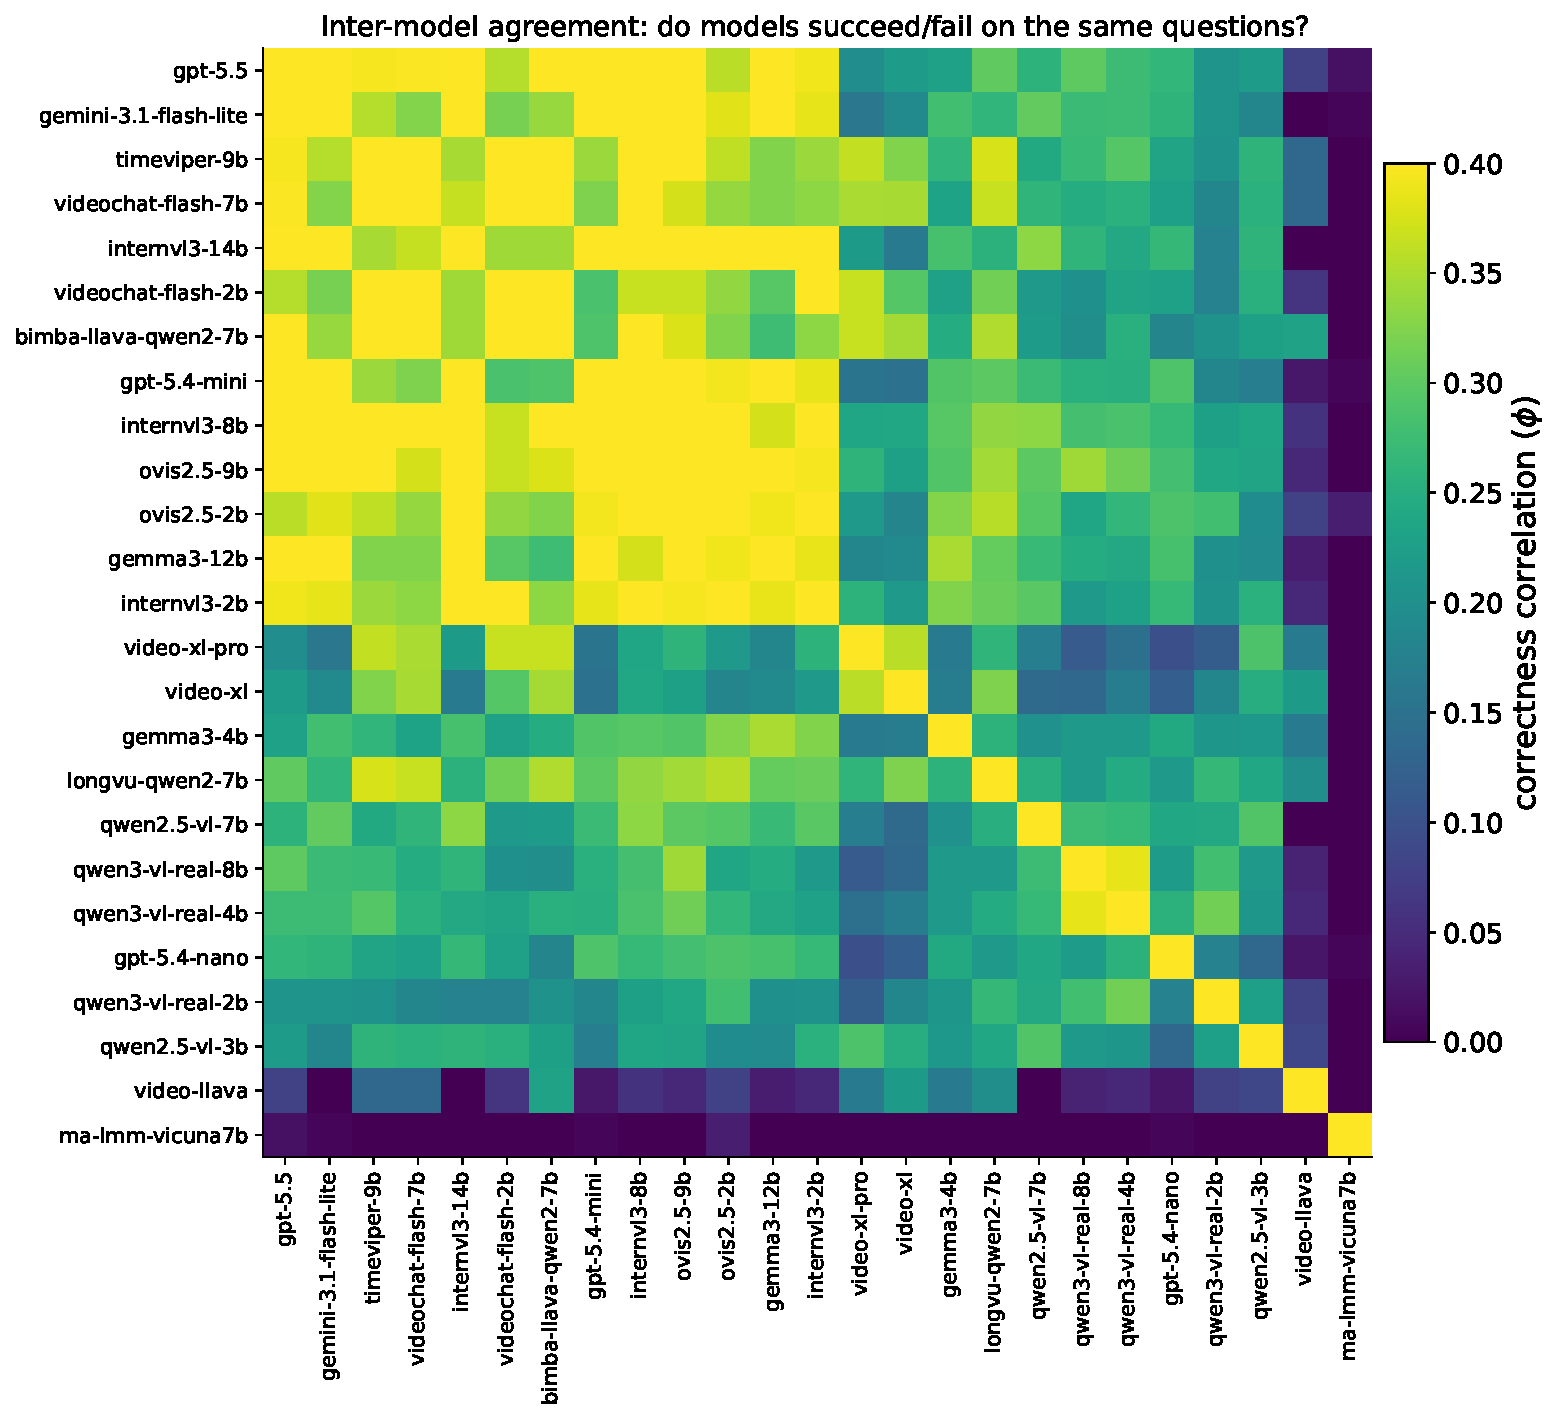
\includegraphics[width=\linewidth]{figures/fig_model_agreement.pdf}
\caption{Inter-model agreement}\label{fig:agree}
\end{subfigure}
\caption{Top, predicted-letter distribution per model, where a uniform column is 12.5\% per letter. Bottom, pairwise correctness correlation between models, mean $\phi=0.24$.}
\label{fig:biasagree}
\end{figure}




\section{Identity conditioning pipelines}
\label{app:reid}
Each pipeline runs three stages before the VLM sees anything. A detector and tracker find and follow every person and animal, a cross-shot linker merges tracklets that belong to the same identity, and a grounding step maps the question referent to one global identity and renders a clip that marks only that identity. We cross four trackers, namely BoT-SORT \citep{botsort}, ByteTrack \citep{bytetrack}, DeepOCSORT \citep{deepocsort}, and StrongSORT \citep{strongsort}, with five linkers, namely generic CLIP features \citep{clip} and the four dedicated re-identification models OSNet \citep{osnet}, CLIP-ReID \citep{clipreid}, TransReID \citep{transreid}, and SOLIDER \citep{solider}, for twenty pipelines in total. CLIP linking is the generic baseline linker. It embeds the cropped frames of each tracklet with a frozen CLIP image encoder \citep{clip}, averages them into one tracklet descriptor, and merges two tracklets when their descriptors exceed a cosine-similarity threshold, so it associates identities by general visual appearance rather than by a representation trained for re-identification. The four dedicated models replace this generic embedding with a re-identification embedding trained to be invariant to pose, viewpoint, and background, and are otherwise dropped into the same link-by-threshold step. Every pipeline is evaluated with all seventeen local models on a common question set, and Table~\ref{tab:reid} reports the mean over those models.

The highlighted raw-video row at 19.67\% sits above every pipeline, so handing the model a clean identity track hurts rather than helps. The spread across trackers never exceeds 0.6 points, which shows the result is not an artifact of one weak tracker, and the dedicated re-identification models are marginally worse than generic CLIP linking, which shows stronger identity embeddings do not translate into better answers. We read this as evidence that capable VLMs exploit scene context that a single-identity crop removes, and that identity association is not the operation the benchmark is bottlenecked on. The grounding step is oracle-free, since the referent phrase is matched to a global identity by the same features that link tracklets, so no pipeline ever sees the correct answer. Rendering marks only the grounded identity by suppressing other regions, which is precisely the intervention that strips the scene context capable models rely on.




\begin{table}[h]
\centering
\caption{Accuracy averaged over seventeen VLMs on a common subset, for five identity-linking methods crossed with four trackers. The raw-video baseline is highlighted, and every pipeline sits at or below it.}
\label{tab:reid}
\small
\begin{tabular}{@{}lccccc@{}}
\toprule
\rowcolor{sectiongray}
\multicolumn{6}{c}{\textbf{Generic feature linking}} \\
\midrule
Method & BoT-SORT & ByteTrack & DeepOCSORT & StrongSORT & Mean \\
CLIP linking & 19.00 & 18.94 & 18.70 & 18.90 & \textbf{18.89} \\
\midrule
\rowcolor{sectiongray}
\multicolumn{6}{c}{\textbf{Dedicated re-identification models}} \\
\midrule
OSNet & 18.60 & 18.43 & 18.70 & 18.56 & 18.57 \\
CLIP-ReID & 18.82 & 18.47 & 18.23 & 18.65 & 18.54 \\
TransReID & 18.61 & 18.28 & 18.53 & 18.46 & 18.47 \\
SOLIDER & 18.73 & 18.45 & 18.28 & 18.51 & 18.49 \\
\midrule
\rowcolor{highlightgreen}
Raw video & & & & & \textbf{19.67} \\
\bottomrule
\end{tabular}
\end{table}

\begin{figure}[h]
\centering
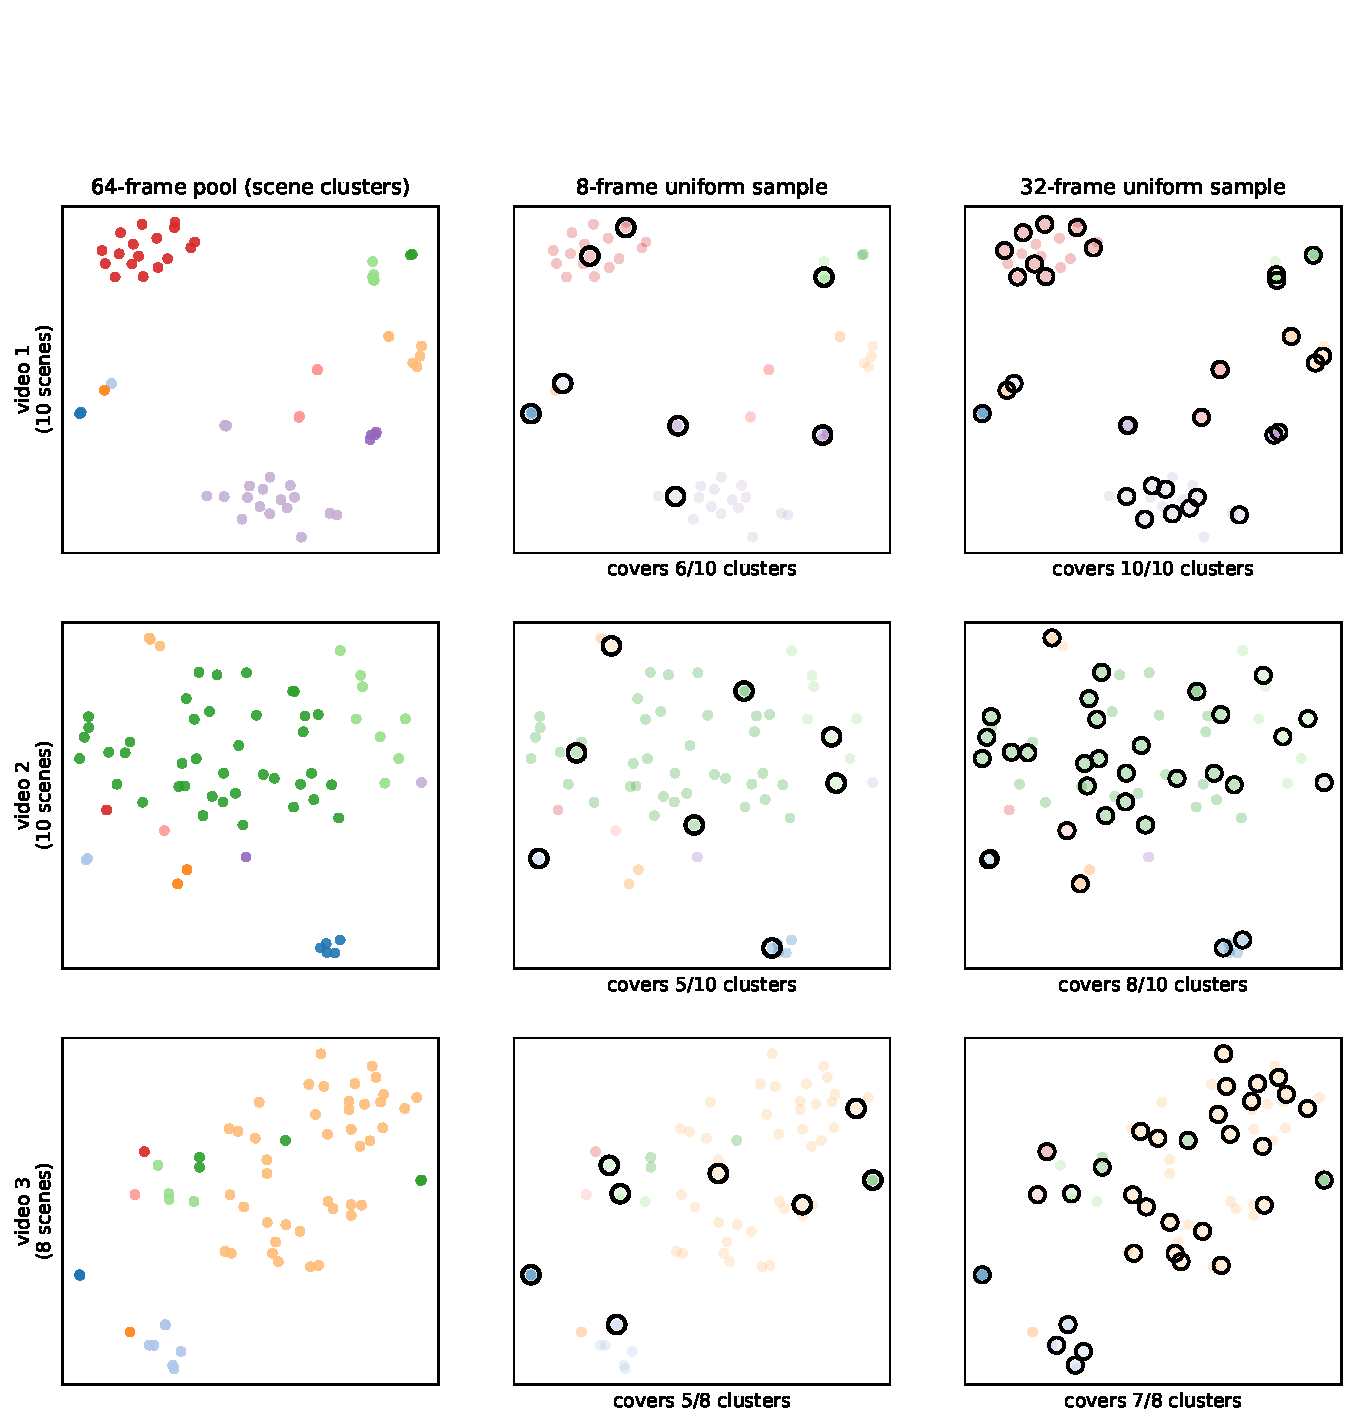
\includegraphics[width=0.8\linewidth]{figures/fig_tsne_collapse.pdf}
\caption{t-SNE of a 64-frame pool per video, where colors are scene clusters and markers show which clusters an 8-frame and a 32-frame uniform sample reach. The uncovered clusters visualize the coverage gap that Figure~\ref{fig:collapse} quantifies.}
\label{fig:tsne}
\end{figure}

\section{Selection probe and prior-work reconciliation}
\label{app:extra}
The selection probe scores 64 candidate frames per video against the question text with a CLIP encoder and keeps the eight highest-scoring frames, without any training. Figure~\ref{fig:clip} shows the per-model lift over uniform sampling at a fixed eight-frame budget, split into a question-conditioned variant that scores against the full question and a referent-conditioned variant that scores against the referent phrase only. Both variants raise accuracy on full-fidelity models by 1.0 to 2.7 points, which confirms that the right eight frames beat eight uniform frames. The one model that loses accuracy is VideoChat-Flash, which performs its own internal frame selection, so an external selector conflicts with its native handling and selection must instead be integrated inside the model.

Table~\ref{tab:prior} reconciles our numbers with published claims on the same source videos. A model family that reports 87.5\% on original MovieChat-1k questions and a token-compression model that exceeds 95\% on needle-in-a-haystack retrieval both fall below 20\% on \bench, which shows the gap is not explained by video difficulty or by the models being weak in general. The common factor is that prior tasks reward coarse retrieval and global gist, while \bench{} requires reading a fine-grained attribute of a tracked referent. Scale, which helps on many prior suites, is uncorrelated with accuracy here at $r=0.05$, which is the last row of the table. The selector is training-free and adds no parameters, so its lift is a lower bound on what a learned in-model selector could reach. The prior-work rows quote published numbers on the same source videos rather than re-runs, so they establish a task gap rather than a controlled ablation.

\begin{table}[t]
\centering
\caption{Published long video claims against \bench. The same source videos and models drop sharply once questions require identity-grounded reading.}
\label{tab:prior}
\small
\begin{tabular}{@{}lcc@{}}
\toprule
Setting & Published & \bench \\
\midrule
MovieChat-1k original QA (HierarQ) & 87.5 & \textless 20 \\
Needle-in-a-haystack (Video-XL-Pro) & \textgreater 95 & 18--19 \\
Long video suites, strong systems & \textgreater 80 & 29.5 best \\
Scale helps accuracy & yes & $r=0.05$ \\
\bottomrule
\end{tabular}
\end{table}


\begin{figure}[h]
\centering
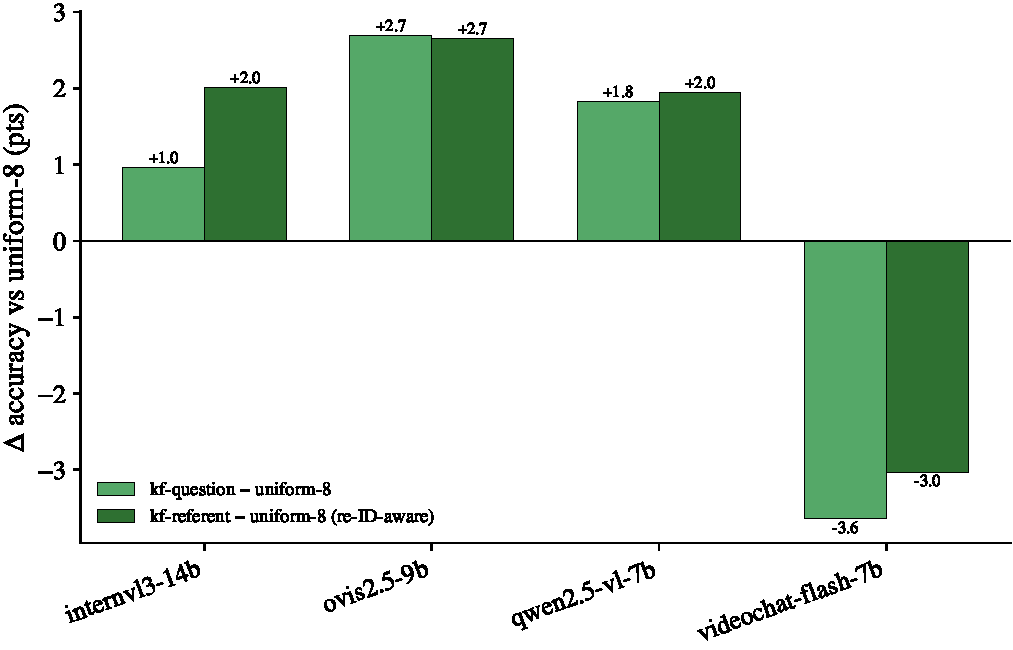
\includegraphics[width=0.8\linewidth]{figures/fig_clip_keyframe_delta.pdf}
\caption{Lift of CLIP keyframe selection over uniform sampling per model. External selection hurts the model with native internal frame handling.}
\label{fig:clip}
\end{figure}

\section{Difficulty drivers across video properties}
\label{app:drivers}
The main text rejects identity confusion as the source of difficulty using two proxies, so this appendix widens the test to every measurable video property. If difficulty were driven by how visually complex a video is, per-video accuracy would fall as duration, cuts, and variability rise, and if it were driven by identity confusion it would fall as concurrent people and identity-switch opportunity rise. We compute per-video accuracy averaged over all \nummodels{} models and correlate it against five properties, with quintile means overlaid in Figure~\ref{fig:driversmulti}. Difficulty rises slightly with duration at $r=+0.43$, scene cuts at $r=+0.31$, and visual variability at $r=+0.42$, and it is uncorrelated with the two identity-confusion proxies, at $r=+0.02$ for maximum concurrent people and $r=+0.03$ for identity-switch opportunity. The positive signs mean longer and more varied videos are marginally easier, not harder, and the near-zero identity proxies mean crowding a scene with people does not raise difficulty. This reinforces the main-text conclusion that the bottleneck is temporal coverage rather than identity confusion. Identity-switch opportunity counts frames where two tracked identities cross or exchange screen position, so it is a direct proxy for the confusion the benchmark name suggests, and its near-zero correlation is the cleanest single rejection of the identity-confusion reading. The positive duration and cut correlations are weak enough that they set no usable difficulty prior.
\begin{figure}[t]
\centering
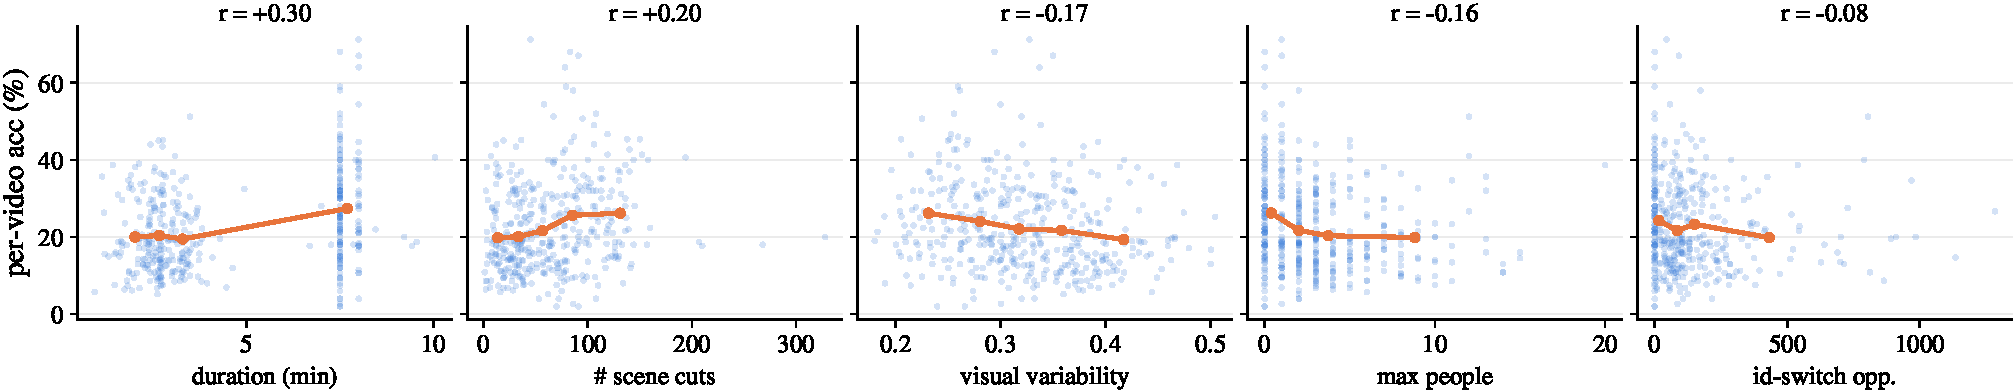
\includegraphics[width=\linewidth]{figures/fig_drivers_multi.pdf}
\caption{Per-video accuracy over \nummodels{} models against five video properties, with quintile means overlaid. Duration, scene cuts, and visual variability carry weak positive correlations, while the identity-confusion proxies of concurrent people and identity-switch opportunity are uncorrelated with difficulty.}
\label{fig:driversmulti}
\end{figure}

\section{Question-side difficulty}
\label{app:qhardness}
Difficulty could live in the question text rather than the video, so we test whether wording, referral strategy, or referent type predicts accuracy. If long or particular phrasings were the obstacle, accuracy would track question length or a single referral strategy. We measure accuracy against three question-side factors in Figure~\ref{fig:qhardness}. Accuracy is flat against question length at Pearson $r=+0.02$, so wordier questions are not harder. Accuracy across the five well-supported referral strategies spans a narrow 17.6 to 19.4 band, with activity at 19.4, mixed at 18.4, environment at 18.2, location at 18.1, and appearance at 17.6, so how the referent is named barely changes difficulty. Splitting by referent type through a keyword proxy, since no referent-type metadata tag exists, gives person referents 18.1\% at $n=2648$ against animal referents 19.5\% at $n=913$, so animal referents are marginally easier. No question-side factor concentrates the difficulty, which points back to the visual tracking demand as the shared cause. The referent-type split uses a keyword proxy rather than a metadata tag, so its person and animal counts are approximate and the 1.4-point gap is read as directional. No question-side factor exceeds a weak correlation, which rules out phrasing as a hidden text-only shortcut the committee missed.
\begin{figure}[t]
\centering
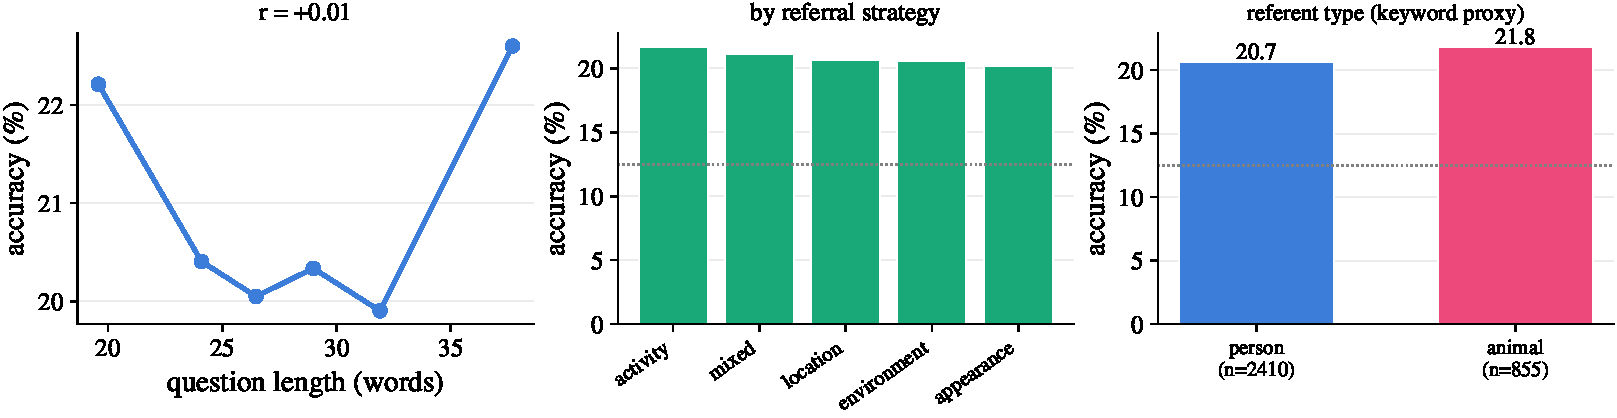
\includegraphics[width=\linewidth]{figures/fig_question_hardness.pdf}
\caption{Question-side difficulty. Left, accuracy against question length is flat at $r=+0.02$. Middle, accuracy by referral strategy spans a narrow 17.6 to 19.4 band. Right, a keyword proxy for referent type gives person 18.1\% and animal 19.5\%.}
\label{fig:qhardness}
\end{figure}

\section{Coverage across models}
\label{app:covmulti}
The main text shows coverage helps InternVL3-14B, so this appendix checks that the coverage lever generalizes across the model set rather than being one family's quirk. We sweep the uniform frame budget from 8 to 64 for seven full-fidelity models in Figure~\ref{fig:covmulti}. Coverage helps most models, with InternVL3-14B gaining 3.2 points and Qwen2.5-VL-7B gaining 3.1 points from 8 to 32 frames, and one model, Qwen3-VL-8B, stays flat across the sweep. InternVL3-8B and InternVL3-14B have no valid 64-frame point because that run broke, so their curves stop at 32 frames. The consistent upward slope across families confirms that added temporal coverage, not a single architecture, is the shared lever, while the one flat model marks the ceiling of what uniform coverage alone can buy. The sweep holds every other setting fixed, so the slope isolates temporal coverage from resolution and prompt. The flat model marks where uniform coverage alone stops paying, which is the exact gap the query-conditioned selection of Section~\ref{sec:method} targets.
\begin{figure}[t]
\centering
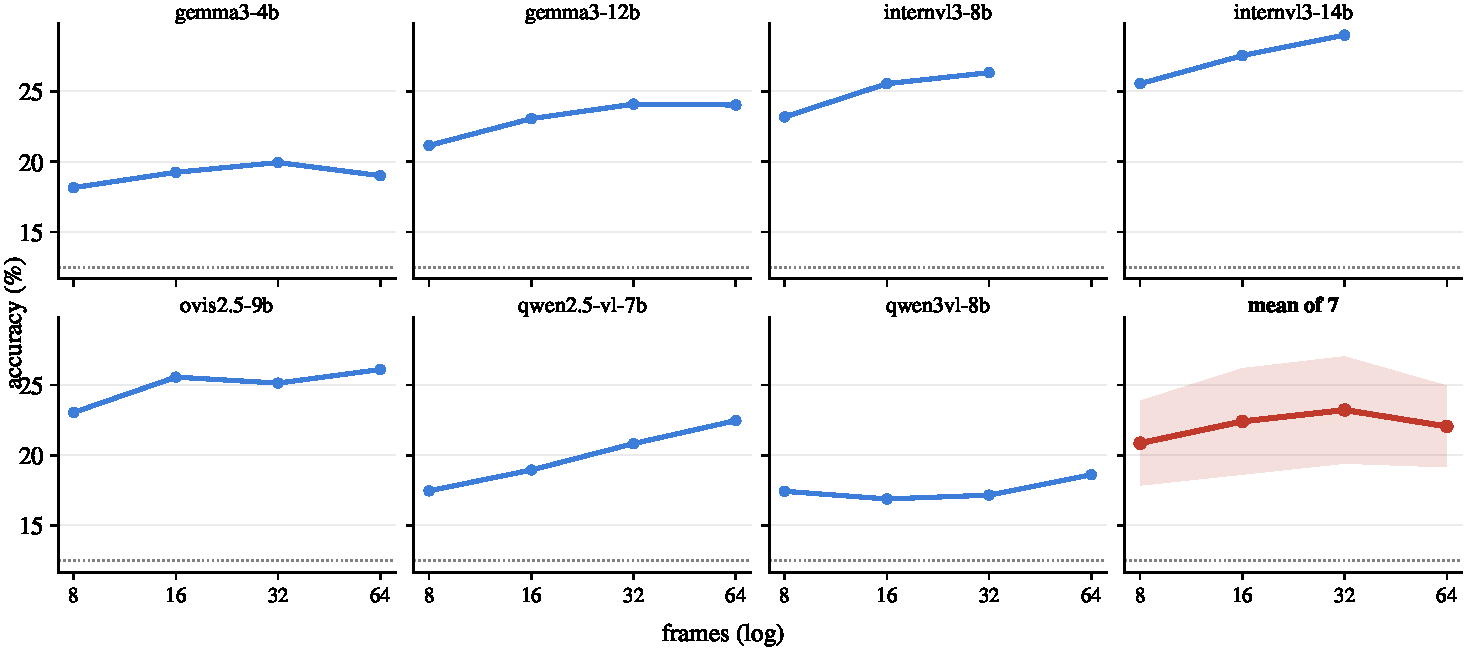
\includegraphics[width=0.92\linewidth]{figures/fig_coverage_multimodel.pdf}
\caption{Accuracy against uniform frame budget for seven full-fidelity models, one panel each. Most models rise with more frames, InternVL3-14B by 3.2 points and Qwen2.5-VL-7B by 3.1 points from 8 to 32 frames, while Qwen3-VL-8B is flat. The InternVL3-8B and 14B curves stop at 32 frames because the 64-frame run broke.}
\label{fig:covmulti}
\end{figure}

\section{Scaling within families}
\label{app:scalefamily}
The main text reports a weak parameter-to-accuracy correlation of 0.05 across all models, which could hide a strong within-family trend masked by family differences. We plot accuracy against parameter count with a separate line per family in Figure~\ref{fig:scalefamily}. Scaling inside a family adds a few points at most, and the vertical gaps between family lines exceed the slope along any one of them, so family identity dominates parameter count. This within-family view echoes the main-text $r=0.05$ and shows that the weak overall correlation is not an averaging artifact but a real ceiling on what scale delivers for this skill. Reading slope within a family removes the confound that families differ in data and training recipe, which an all-model regression would fold into the trend. The residual within-family slope stays under a few points, so parameter count is not a hidden lever masked by family mixing.
\begin{figure}[t]
\centering
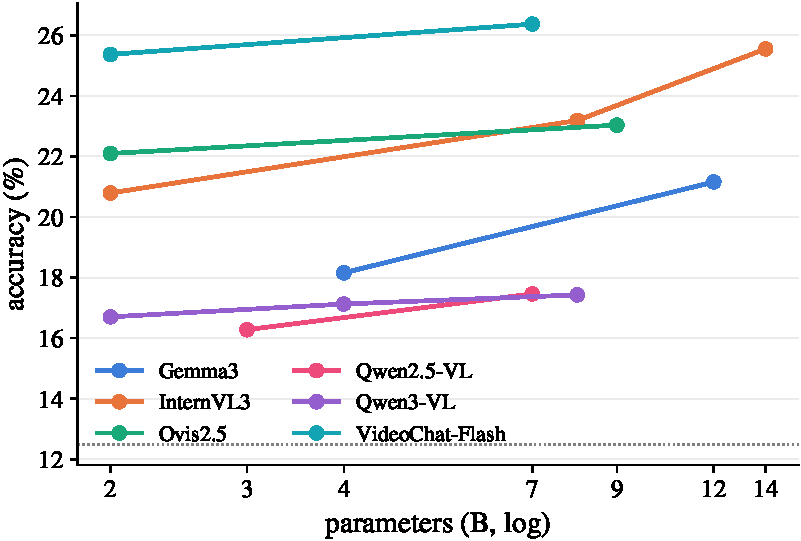
\includegraphics[width=0.62\linewidth]{figures/fig_scaling_family.pdf}
\caption{Accuracy against parameter count with a within-family line per model family. Scaling inside a family adds a few points at most, and family identity dominates parameter count, echoing the main-text correlation of 0.05.}
\label{fig:scalefamily}
\end{figure}

\section{Per-challenge coverage gain}
\label{app:perchalcov}
Coverage helps unevenly across challenge types in Section~\ref{sec:necessity}, so this appendix quantifies which challenge types gain the most from added frames. We compute the mean accuracy gain from 1 to 8 frames for each challenge type, averaged over the four frame-control models, and render it as a one-row heatmap in Figure~\ref{fig:perchalcov}. The types that require re-locating an identity after it leaves view, namely occlusion recovery and disambiguation among similar identities, gain the most from added frames, while types answerable from a single reference frame gain little. This localizes the coverage benefit to exactly the tracking-heavy skills the benchmark targets, so the coverage lever acts where the benchmark is hardest. The gain is measured from 1 to 8 frames, so it captures the move from a single reference frame to a short temporal window rather than the full sweep. Occlusion recovery and disambiguation gain most because their answer frame is often absent from a single-frame sample, which is the coverage failure the main text names.
\begin{figure}[t]
\centering
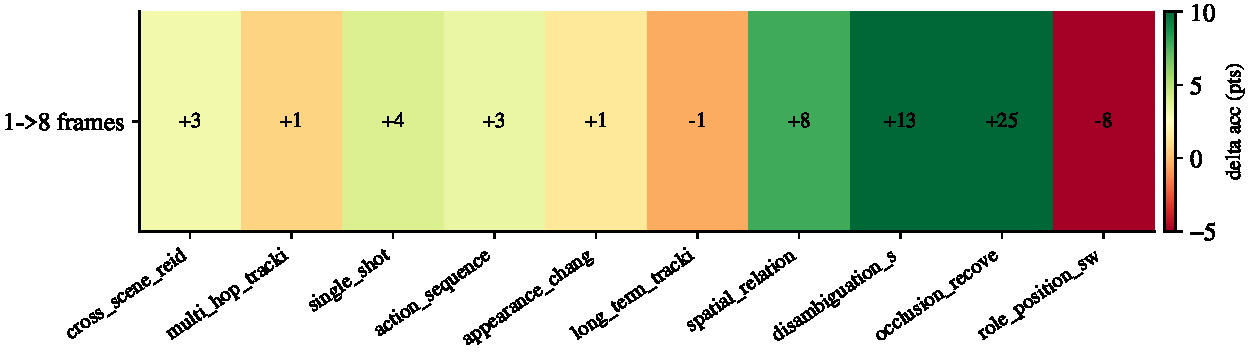
\includegraphics[width=0.92\linewidth]{figures/fig_perchallenge_coverage.pdf}
\caption{Mean accuracy gain from 1 to 8 frames per challenge type, averaged over the four frame-control models. Types that require re-locating a lost identity gain the most from added frames.}
\label{fig:perchalcov}
\end{figure}

\section{Robustness batteries}
\label{app:corruption}
Section~\ref{sec:necessity} summarizes three robustness probes, and this appendix shows each in full on the four frame-control models. The probes matter because a benchmark whose answers survive frame shuffling or option rotation would be measuring a shortcut rather than temporal reading, so we test frame order, option order, and input corruption directly.

Frame order carries a weak signal that shrinks with scale. Figure~\ref{fig:torder} shows that shuffling or reversing the eight frames lowers InternVL3-2B by 1.8 to 2.8 points, while the effect reaches about zero for InternVL3-14B. Option order barely moves accuracy yet flips the chosen answer often. Figure~\ref{fig:optsens} shows that rotating the option contents by three positions leaves accuracy near flat while the model changes its content answer on 49.8\% of questions, so accuracy stability hides an unstable choice. Both results are consistent with models reading frames as a loosely ordered set rather than a tracked sequence, which matches the tracking failures in Section~\ref{sec:skills}.
Input corruption lowers accuracy while losing pixels does not. If the benchmark were solvable from coarse global cues, mild corruption would leave accuracy untouched, so we probe six corruptions against a clean baseline. We apply blur, JPEG, Gaussian noise, low light, motion blur, and downscaling to 112 pixels at a fixed reduced-resolution probe setting, shown in the main-text Figure~\ref{fig:robbattery}(c). Because the clean baseline itself runs at reduced resolution, the panels report relative drops rather than absolute accuracy. Corruption lowers accuracy by up to 4.5 points, moving InternVL3-2B from 17.8\% clean to 13.2\% under noise, while downscaling to 112 pixels is nearly lossless. The pattern matches the weak per-frame resolution effect in Section~\ref{sec:coverage}, since losing pixels barely hurts while losing signal content does, which is consistent with coverage rather than fidelity being the bottleneck. Because these probes ablate one factor at a time against a shared clean baseline, they isolate whether each corruption removes benchmark-relevant signal, and only content-destroying corruptions do.

\section{Visual content landscape}
\label{app:landscape}
A natural worry is that difficulty is tied to a particular kind of video, such as dark or crowded footage, which would make \bench{} a test of one visual regime rather than of identity-grounded reading. We embed every video by its mean CLIP frame feature, project the set with t-SNE, and color each point by per-video accuracy averaged over all \nummodels{} models in Figure~\ref{fig:landscape}. Accuracy is mixed across the visual-content clusters with no accuracy tiers, so easy and hard videos sit side by side within every cluster and difficulty is not tied to a particular visual video type. This contrasts honestly with robustness studies that report clean accuracy tiers by content, and it means \bench{} difficulty is a property of the identity-grounded question rather than of the footage it is asked over. Coloring by per-video accuracy rather than by content lets any cluster reveal an accuracy tier it carries, and none appear. This is a stronger control than reporting mean accuracy per content bin, since it would expose even a small pocket of uniformly hard footage.
\begin{figure}[t]
\centering
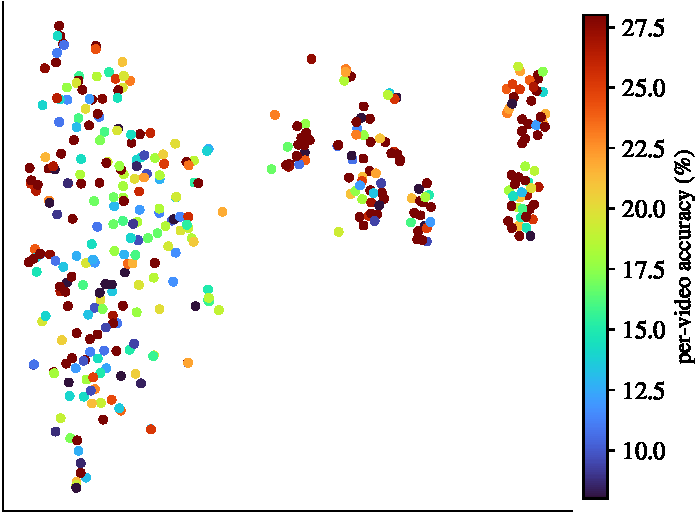
\includegraphics[width=0.46\linewidth]{figures/fig_video_landscape.pdf}
\caption{t-SNE of every video by mean CLIP frame embedding, colored by per-video accuracy over \nummodels{} models. Accuracy is mixed within every visual-content cluster with no accuracy tiers, so difficulty is not tied to a particular visual video type.}
\label{fig:landscape}
\end{figure}

\end{document}
